% wealth_garch_theory.tex, the manuscript of the theory paper of papers/wealth_garch.
% Created 23 October 2026 as pass 1 of the plan in TODO.md (item PLAN),
% following papers/MANUSCRIPT_SKELETON.md, with
% papers/subjective_racism/paper_a/skeleton_ClassMarkers.tex as the
% reference. Filled the same day with the theoretical rows of the parent
% MANUSCRIPT.tex (author, 23 October 2026: the theory paper rests only on
% its theoretical novelty). TODO.md maps each row to its parent row.
%
% STRUCTURE THE CHECKER RELIES ON (checks/verify_manuscript.py)
%   Rows are written only through the six row macros below, and proofs only
%   through the mproof environment. IDs are K1, K2, ... (introduction),
%   P1, ... (players), A1, ... (assumptions), M1, ... (model), L1, ... (literature)
%   and C1, ... (conclusions).
%     \krow{ID}{headline}{model rows}{scope note}
%     \prow{ID}{player}{choice faced}{how the model settles it}{in the literature}{rows}
%     \arow{ID}{assumption}{in plain English}{symbols}{model rows}{reason}
%     \mrow{ID}{claim in words}{statement in symbols}{Lean theorems}
%     \lrow{ID}{bib key}{what we rely on}{verbatim quote}{page}{model rows}
%     \crow{ID}{statement}{model or literature rows}
%     \begin{mproof}{model row}{Lean theorems} ... \end{mproof}
%   Lists of rows or theorems are comma-separated. Lean theorem names are the
%   fully qualified names declared under theory/lean/.
%
% RULES THE CHECKER ENFORCES
%   Introduction rows point to model rows only. Player rows and conclusion rows
%   point to model or literature rows only. Assumption rows point to model rows
%   only, and every model row rests on at least one assumption. Every model row
%   names Lean theorems that exist in an audited Lean file and has exactly one
%   proof in Appendix A naming the same theorems. Every literature row's quote
%   appears verbatim in the paper's lit/ record. In every proof, plain English
%   is at most 30% of the text, measured as prose words over prose words plus
%   mathematical tokens. Every section and table of the skeleton is present,
%   found by its label.
\documentclass[11pt]{article}
\usepackage[T1]{fontenc}
\usepackage[utf8]{inputenc}
\usepackage{mathptmx}
\usepackage{microtype}
\usepackage[a4paper,margin=1.8cm]{geometry}
\usepackage{amsmath,amssymb,amsthm}
\usepackage{booktabs}
\usepackage{array}
\usepackage{longtable}
\usepackage{url}
\usepackage[hidelinks]{hyperref}
\usepackage{natbib}
\usepackage[scaled=0.92]{helvet}
\usepackage{graphicx}
\usepackage[export]{adjustbox}
\usepackage{pdflscape}
\usepackage{float}
\usepackage{tikz}
\usetikzlibrary{arrows.meta,fit,calc,backgrounds}
% ledger_styles.tex, the TikZ styles of the four ledger figures of
% wealth_garch_theory.tex (Figures 1 to 4). Agents are green, objects blue,
% counterparties orange, the regulator red, preference-driven agents violet,
% and what is not an agent of the model grey and dashed. Solid arrows are
% derived (a model row, or a paper's result its Lean record proves), dashed
% arrows are assumed or taken as given, dotted arrows are stated in words or
% open.
\tikzset{
  >={Stealth[length=2.2mm]},
  ledger/.style={every node/.style={font=\small}},
  agent/.style={draw=black!60, line width=0.6pt, align=center, text width=4.0cm, minimum height=3.0cm, inner sep=5pt, rounded corners=4pt, fill=green!10},
  object/.style={draw=black!60, line width=0.6pt, align=center, text width=3.8cm, minimum height=2.6cm, inner sep=5pt, rounded corners=4pt, fill=blue!10},
  other/.style={draw=black!60, line width=0.7pt, align=center, text width=4.4cm, minimum height=3.0cm, inner sep=5pt, rounded corners=4pt, fill=orange!15},
  regulator/.style={other, fill=red!10},
  pref/.style={other, fill=violet!10},
  outside/.style={draw=black!50, dashed, align=center, text width=4.0cm, minimum height=1.8cm, inner sep=4pt, fill=black!5},
  lab/.style={font=\scriptsize, align=center, fill=white, inner sep=1.2pt, text width=3.4cm},
  settled/.style={->, line width=0.6pt},
  given/.style={->, line width=0.6pt, dashed},
  open/.style={->, line width=0.6pt, dotted, line cap=round},
}


\emergencystretch=1.5em
% Characters that appear verbatim in quotations of the lit/ records.
\DeclareUnicodeCharacter{2217}{\ensuremath{^*}}
\DeclareUnicodeCharacter{03C0}{\ensuremath{\pi}}
\DeclareUnicodeCharacter{2264}{\ensuremath{\le}}
\DeclareUnicodeCharacter{2212}{\ensuremath{-}}
\DeclareUnicodeCharacter{2206}{\ensuremath{\Delta}}
\DeclareUnicodeCharacter{00B5}{\ensuremath{\mu}}
\DeclareUnicodeCharacter{03C1}{\ensuremath{\rho}}
\DeclareUnicodeCharacter{03B3}{\ensuremath{\gamma}}
\DeclareUnicodeCharacter{03C3}{\ensuremath{\sigma}}
\DeclareUnicodeCharacter{03BA}{\ensuremath{\kappa}}
\DeclareUnicodeCharacter{2032}{\ensuremath{'}}

\newcolumntype{P}[1]{>{\raggedright\arraybackslash}p{#1}}

\urlstyle{tt}
\makeatletter
\g@addto@macro\UrlBreaks{\do\.\do\_\do\,}
\makeatother
\newcommand{\lean}[1]{\path{#1}}
\newcommand{\mm}[6]{#1 & \textbf{#2} & #3 & #4 & #5 & #6 \\ \addlinespace}
\newcommand{\rowref}[1]{#1}
\newcommand{\unv}[1]{\textit{Unverified:} #1}
\newcommand{\pend}[1]{\textit{Pending:} #1}

\newcommand{\krow}[4]{#1 & #2 & \rowref{#3} & #4 \\ \addlinespace}
\newcommand{\prow}[6]{#1 & #2 & #3 & #4 & #5 & \rowref{#6} \\ \addlinespace}
\newcommand{\arow}[6]{#1 & #2 & #3 & #4 & \rowref{#5} & #6 \\ \addlinespace}
\newcommand{\mrow}[4]{#1 & #2 & #3 & \lean{#4} & p.~\pageref{proof:#1} \\ \addlinespace}
\newcommand{\lrow}[6]{#1 & \citet{#2} & #3 & ``#4'' & #5 & \rowref{#6} \\ \addlinespace}
\newcommand{\crow}[3]{#1 & #2 & \rowref{#3} \\ \addlinespace}

\newenvironment{mproof}[2]
  {\subsection*{Proof of #1}\label{proof:#1}%
   {\raggedright\noindent\textit{Lean:} \lean{#2}.\par}\smallskip}
  {\par\hfill$\square$\par\medskip}

% Working title, from papers/wealth_garch/MANUSCRIPT.tex. The author sets
% the title.
\title{Asymmetric Capital Buffer Control}
\author{}
\date{Manuscript skeleton, 23 October 2026}

\begin{document}
\maketitle

\section{Introduction}
\label{sec:intro}

\subsection{Question}

% The question is the literature's, as Section~\ref{sec:literature} traces it,
% reassessed against the measurement map of Appendix~\ref{app:terms}.
When a bank's capital buffer is explained by a fixed issuance cost together
with a shortfall penalty that grows as equity falls below required capital,
does the bank's policy carry the asymmetry parameter of that penalty separately
from the fixed issuance cost, and if so where, in the dividend barrier and the
recapitalisation trigger or in buffer variance? The asymmetry parameter is
never observed (Appendix~\ref{app:terms}), so it can be read only off what the
policy shows, and at one it switches the shortfall penalty off and leaves the
model with issuance costs alone (M8), so whether it is identified decides whether the
specification \citet{peura2006} call for (L18) can be tested against theirs
rather than imposed (L20). The bank recapitalises by impulse control at a fixed
issuance cost and takes risky exposure under a regulatory cap.

\subsection{Answer}

The shortfall penalty moves the thresholds, the dividend barrier and the
recapitalisation trigger. The asymmetry parameter $\lambda_S$ and the
fixed issuance cost $K$ both raise the dividend barrier (M1). The
recapitalisation trigger rises in $\lambda_S$ and falls in $K$ (M2). Because the
two parameters move the trigger in opposite directions, the Jacobian of the
barrier and the trigger in $(\lambda_S,K)$ is non-singular, so the pair is
locally identified from the two thresholds (M3), under the hypotheses that M4
and Appendix~\ref{app:evidence} list. This is K1 and C1. The thresholds
identify the asymmetry parameter and not whose cost the shortfall penalty is
(Appendix~\ref{app:scope}).
The identification is within the model. The two thresholds are recorded as the
state at a dividend and at an issue, and on the panel the parent bundle read
dividends are paid at every state and issues land at no single target, so
neither is measured there as a threshold (Appendix~\ref{app:terms}).

The shortfall penalty does not move the limits of buffer variance. Where the optimal
exposure binds the cap near the distress boundary and deep in surplus, buffer
variance tends to the deficit limit and the surplus limit, which involve only
the asset volatility, the liability volatility, the return-liability
correlation and the regulatory cap (M10, M11). For every exposure that
complies with the cap, binding or not, buffer variance is bounded by the same
quantities (M12). The asymmetry parameter enters the thresholds and not the
limits of buffer variance. This is K2 and C2, with its scope in C3. The
limits need the cap to bind, and on that panel the recorded exposure sits far
below the cap, so the bound of M12, which needs no binding, is the result that
reaches the data (Appendix~\ref{app:terms}).

\footnotesize
\begin{longtable}{@{}P{0.8cm}P{7.0cm}P{1.9cm}P{6.4cm}@{}}
\caption{Headlines.}\label{tab:headlines}\\
\toprule
ID & Headline & Model rows & Scope note \\
\midrule
\endfirsthead
\toprule
ID & Headline & Model rows & Scope note \\
\midrule
\endhead
\krow{K1}{The asymmetry parameter $\lambda_S$ and the fixed issuance cost $K$ are locally identified from the dividend barrier and the recapitalisation trigger, because both raise the barrier and they move the trigger in opposite directions.}{M1, M2, M3, M4}{Local identification from the thresholds, not an estimator. Rests on the hypotheses of Appendix~\ref{app:evidence}, among them the verification theorem, the envelope identities, the signs of $W'(x_L)$ and $N'$, $\Psi(x_L)>0$ and $\rho_L>\mu'(y^*)$. Fails if the two parameters moved the trigger in the same direction (M3). It identifies the asymmetry parameter, not whose cost the shortfall penalty is (L19, Appendix~\ref{app:scope}). The thresholds are recorded as the state at a dividend and at an issue, and on the panel the parent bundle read neither behaves as a threshold (Appendix~\ref{app:terms}), so the identification is within the model. It needs the recapitalisation trigger above the distress boundary. In the solve of Appendix~\ref{app:evidence} the trigger is interior at 42 of 56 parameter points, and where the fixed issuance cost is large against the asymmetry parameter the bank issues only at the distress boundary, where the trigger cannot move. The fixed issuance cost is charged per unit of liabilities (Appendix~\ref{app:scope}). The responses of the thresholds to the fixed issuance cost alone are not claimed new, since \citet{peura2006} and \citet{daihuangkeppo2019} tabulate them, nor is pinning the fixed issuance cost and a second parameter from moments of the thresholds, which \citet{peura2006} do by calibration (L7, L8, L9).}
\krow{K2}{The asymmetry parameter enters the thresholds and not the limits of buffer variance. Where the optimal exposure binds the regulatory cap near both ends, those limits depend only on the asset volatility, the liability volatility, the return-liability correlation and the regulatory cap, and for every compliant exposure buffer variance is bounded by them.}{M3, M10, M11, M12}{That the optimum binds the cap near both ends is a hypothesis. In the solve of Appendix~\ref{app:evidence} the exposure is at the cap at both thresholds and on 85 percent of the inaction region; the bound M12 needs no binding. The surplus limit needs the liquidity branch to bind deep in surplus, which needs borrowing; \citet{bayraktar2026} take no borrowing as the main banking case, under which it never binds (L2, Appendix~\ref{app:scope}). The constant buffer variance on the solvency branch is not claimed new, since it is the constant log-cushion volatility of capped portfolio insurance \citep{blackperold1992}, L5. The contrast is with that rule, whose slopes are set by preferences (L6), while here they are set by regulation and the liability shock is not hedged. On the panel the parent bundle read the cap does not bind, so only the bound of M12 reaches the data (Appendix~\ref{app:terms}).}
\bottomrule
\end{longtable}
\normalsize

\section{Model}
\label{sec:model}

\subsection{Players}

\footnotesize
\begin{longtable}{@{}P{0.7cm}P{2.0cm}P{3.2cm}P{4.4cm}P{3.4cm}P{1.5cm}@{}}
\caption{Players of the model, the choice each faces and how the rows settle it.}\label{tab:players}\\
\toprule
ID & Player & Choice faced & How the model settles it & In the literature & Rows \\
\midrule
\endfirsthead
\toprule
ID & Player & Choice faced & How the model settles it & In the literature & Rows \\
\midrule
\endhead
\prow{P1}{Bank}{Its risky exposure, the dividend barrier, the recapitalisation trigger and the injection target.}{The thresholds are derived, in their responses to $\lambda_S$ and $K$ (M1 to M4) and in the target's independence of the starting state (M7). The exposure is not derived. M11 takes it at the cap as a hypothesis, and M12 bounds every compliant exposure.}{The bank of \citet{peura2006} and of \citet{daihuangkeppo2019}, with a fixed issuance cost, and of \citet{bayraktar2026}, with the cap.}{M1, M2, M3, M4, M7, M11, M12, L1, L7, L9}
\prow{P2}{Shareholders}{None in the model. They receive dividends and supply each issue at the fixed and the proportional issuance cost.}{A rule taken as given. The objective is their value net of the shortfall penalty, and the bank chooses for them (M8). Finite issuance follows from the fixed issuance cost (M6).}{In \citet{peura2006} the owners choose the issue.}{M6, M8, L7}
\prow{P3}{Creditors}{None. The liabilities carry their own shock.}{State. The liability volatility and the return-liability correlation enter the limits and bounds of buffer variance (M10 to M12).}{No paper read has a liability shock unhedged by the safe asset; in \citet{blackperold1992} the reserve asset tracks the liability.}{M10, M11, M12, L5}
\prow{P4}{Supervisor}{None in the model. It sets required capital and the regulatory cap.}{A rule taken as given (A2). The shortfall penalty below the reference stands for its restrictions, a reading no row derives (Appendix~\ref{app:scope}).}{The cap of \citet{bayraktar2026}. The intervention of \citet{milnewhalley2001}, which the buffer guards against (L16).}{M8, M10, L1, L16}
\bottomrule
\end{longtable}
\normalsize

Figure~\ref{fig:ledger} draws the model as a graph. Its nodes are the agents
and the object they act on, equity, named as in Appendix~\ref{app:terms}, and
its arrows are the actions between them, each labelled by the rows that settle
it. The players of Table~\ref{tab:players} are its agents, with the creditors
drawn as the insured and the uninsured, since they hold the liabilities
differently and the model takes their shock as one block (A1).

\begin{landscape}
\begin{figure}[p]
\centering
\adjustbox{max width=\linewidth, max height=0.80\textheight}{% ledger_paper.tex, Figure 1 of wealth_garch_theory.tex: the paper's own
% ledger, six entities of the bundle ledger and eight actions
% (notes/ledger.md). Labels cite the paper's rows.
\sffamily
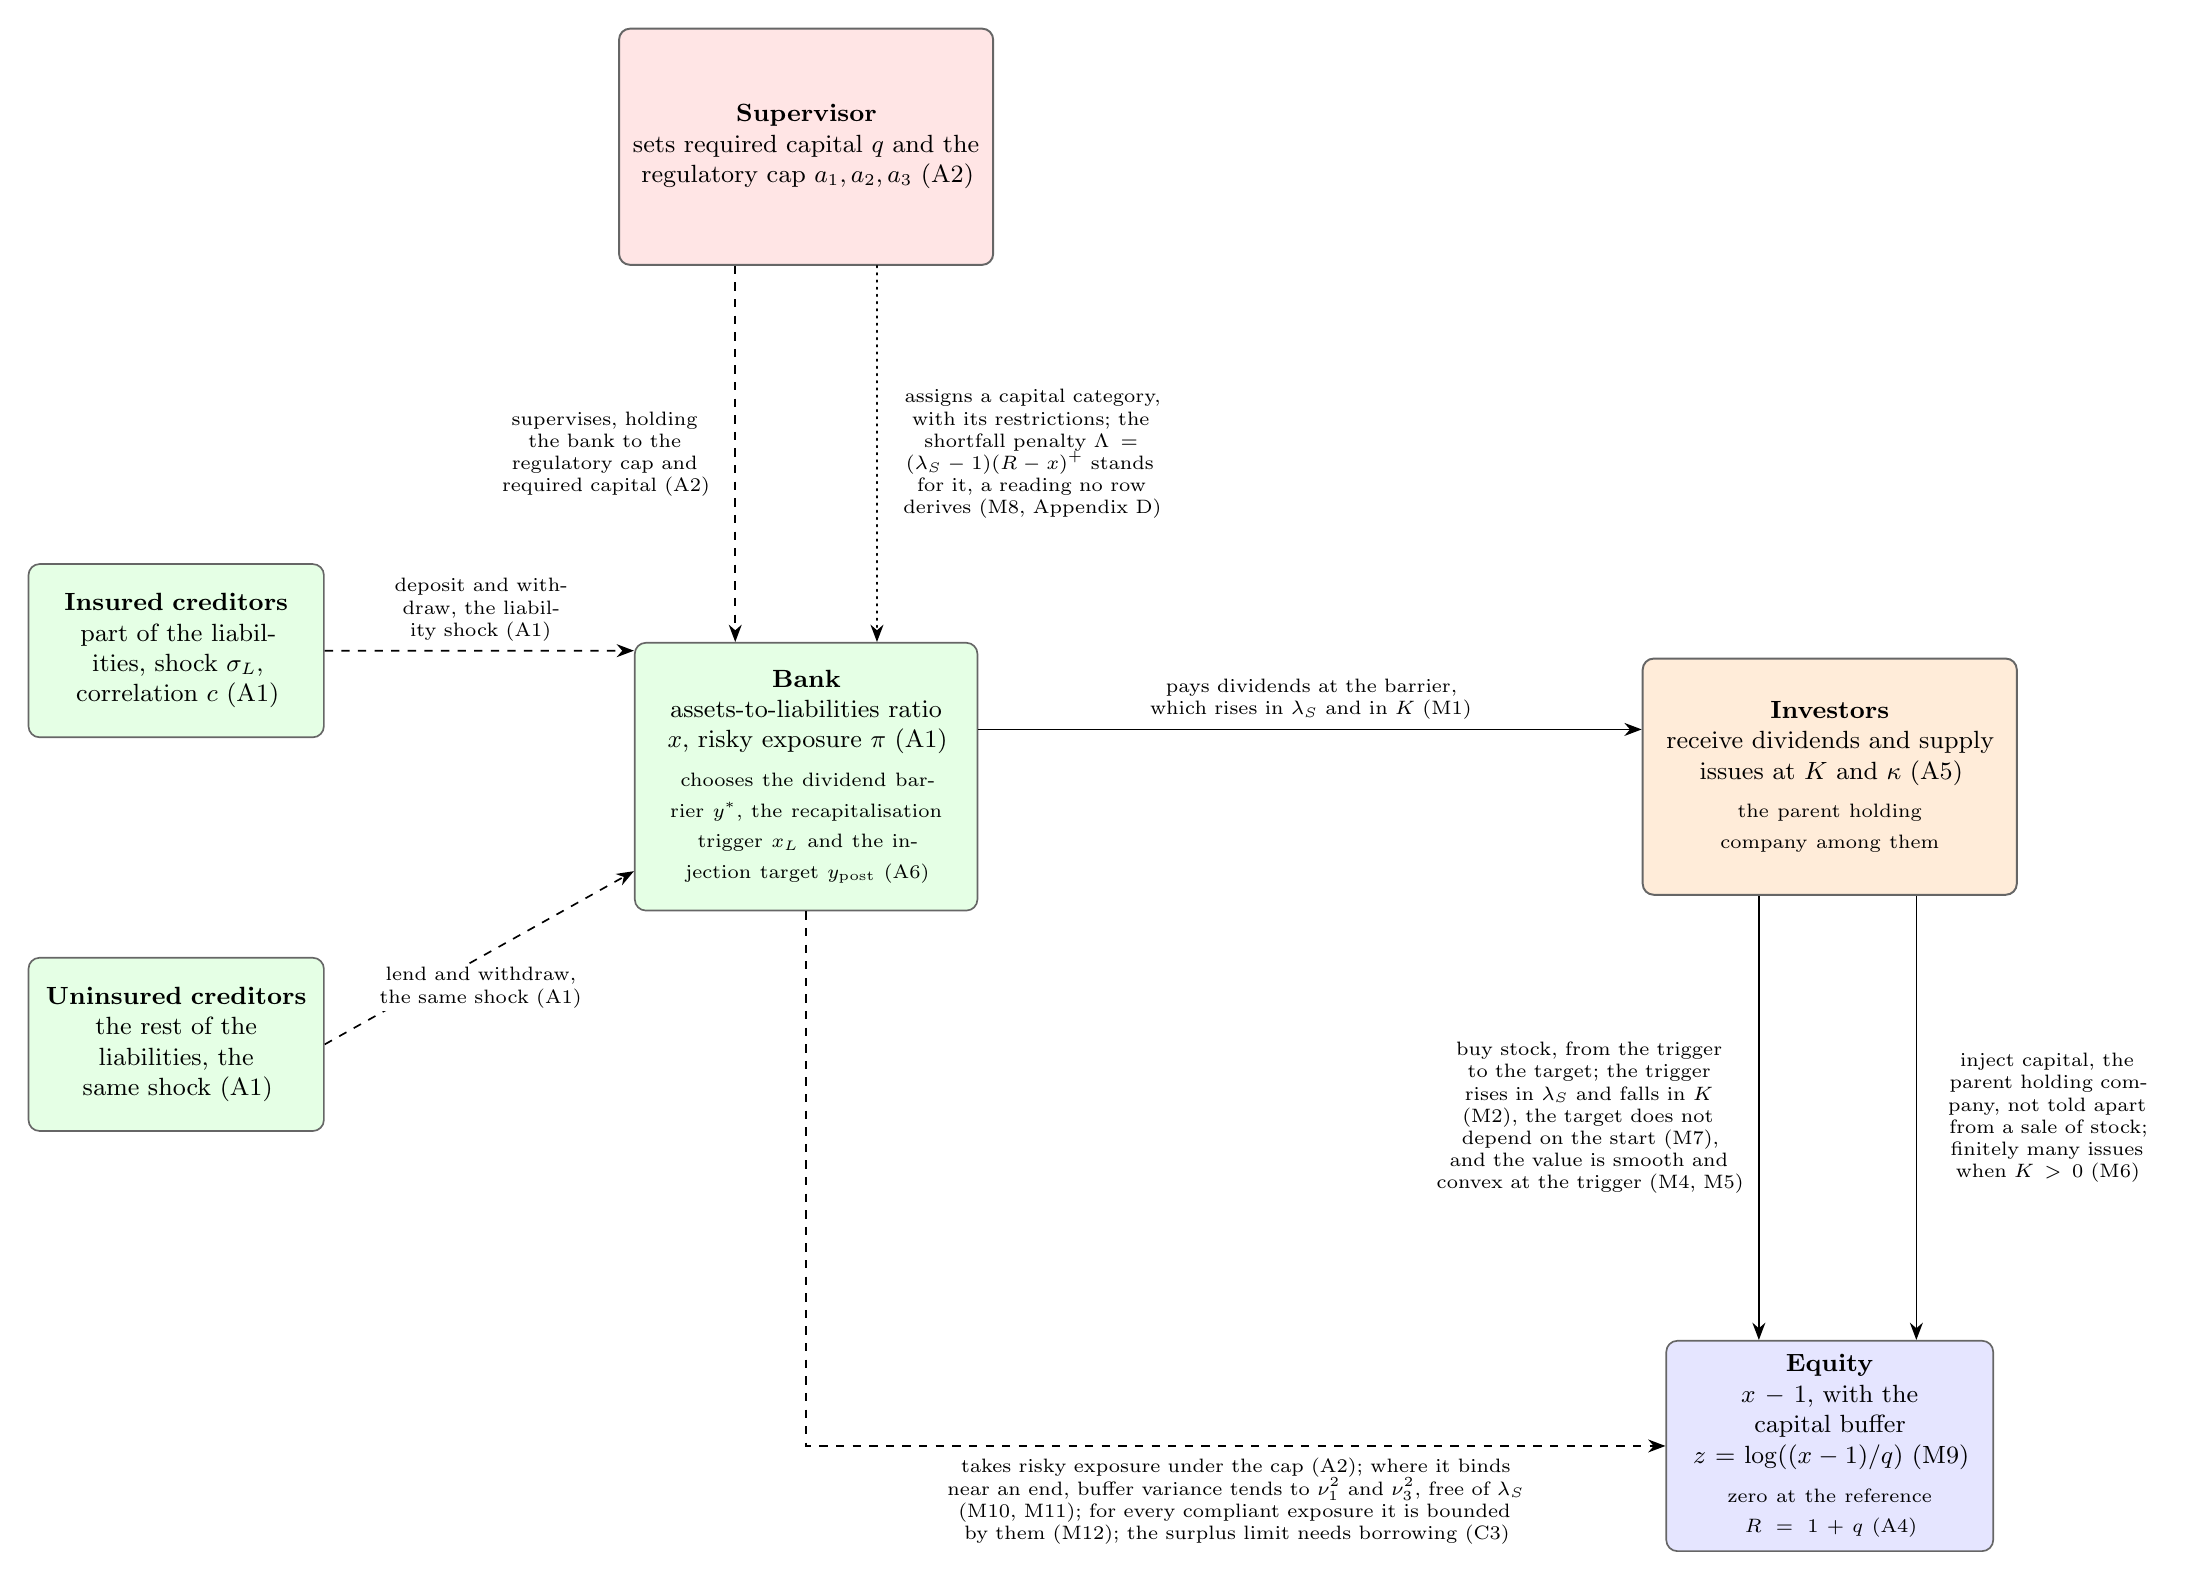
\begin{tikzpicture}[ledger]
\node[regulator] (Sup) at (0,8) {\textbf{Supervisor}\\ sets required capital $q$ and the regulatory cap $a_1,a_2,a_3$ (A2)};
\node[agent, minimum height=3.4cm] (Bank) at (0,0) {\textbf{Bank}\\ assets-to-liabilities ratio $x$, risky exposure $\pi$ (A1)\\[3pt] \scriptsize chooses the dividend barrier $y^*$, the recapitalisation trigger $x_L$ and the injection target $y_{\text{post}}$ (A6)};
\node[other] (Inv) at (13,0) {\textbf{Investors}\\ receive dividends and supply issues at $K$ and $\kappa$ (A5)\\[3pt] \scriptsize the parent holding company among them};
\node[object] (Eq) at (13,-8.5) {\textbf{Equity}\\ $x-1$, with the capital buffer $z=\log((x-1)/q)$ (M9)\\[3pt] \scriptsize zero at the reference $R=1+q$ (A4)};
\node[agent, text width=3.4cm, minimum height=2.2cm] (Ins) at (-8,1.6) {\textbf{Insured creditors}\\ part of the liabilities, shock $\sigma_L$, correlation $c$ (A1)};
\node[agent, text width=3.4cm, minimum height=2.2cm] (Unins) at (-8,-3.4) {\textbf{Uninsured creditors}\\ the rest of the liabilities, the same shock (A1)};

\draw[settled] ([yshift=6mm]Bank.east) -- node[lab, pos=0.5, above=2pt, text width=6.4cm] {pays dividends at the barrier, which rises in $\lambda_S$ and in $K$ (M1)} ([yshift=6mm]Inv.west);
\draw[settled] ([xshift=-9mm]Inv.south) -- node[lab, pos=0.5, anchor=east, xshift=-3pt, text width=4.0cm] {buy stock, from the trigger to the target; the trigger rises in $\lambda_S$ and falls in $K$ (M2), the target does not depend on the start (M7), and the value is smooth and convex at the trigger (M4, M5)} ([xshift=-9mm]Eq.north);
\draw[settled] ([xshift=11mm]Inv.south) -- node[lab, pos=0.5, anchor=west, xshift=3pt, text width=3.0cm] {inject capital, the parent holding company, not told apart from a sale of stock; finitely many issues when $K>0$ (M6)} ([xshift=11mm]Eq.north);
\draw[given]   (Ins.east) -- node[lab, pos=0.5, above=2pt, text width=2.8cm] {deposit and withdraw, the liability shock (A1)} ([yshift=16mm]Bank.west);
\draw[given]   (Unins.east) -- node[lab, pos=0.5, below=2pt, text width=3.0cm] {lend and withdraw, the same shock (A1)} ([yshift=-12mm]Bank.west);
\draw[given]   (Bank.south) |- node[lab, pos=0.75, below=3pt, text width=7.4cm] {takes risky exposure under the cap (A2); where it binds near an end, buffer variance tends to $\nu_1^2$ and $\nu_3^2$, free of $\lambda_S$ (M10, M11); for every compliant exposure it is bounded by them (M12); the surplus limit needs borrowing (C3)} (Eq.west);
\draw[given]   ([xshift=-9mm]Sup.south) -- node[lab, pos=0.5, anchor=east, xshift=-3pt, text width=3.0cm] {supervises, holding the bank to the regulatory cap and required capital (A2)} ([xshift=-9mm]Bank.north);
\draw[open]    ([xshift=9mm]Sup.south) -- node[lab, pos=0.5, anchor=west, xshift=3pt, text width=3.6cm] {assigns a capital category, with its restrictions; the shortfall penalty $\Lambda=(\lambda_S-1)(R-x)^+$ stands for it, a reading no row derives (M8, Appendix~D)} ([xshift=9mm]Bank.north);
\end{tikzpicture}
}
\caption{The paper's ledger. Six entities, the agents in green and orange, the
supervisor in red and equity in blue, and eight actions. Solid arrows are
settled by model rows, dashed arrows are rules or inputs taken as given, and
the dotted arrow is open. Each label cites the rows that settle the action.
The insurer is not drawn, since no row bears on it. K1 concerns the dividend
arrow and the two issue arrows together (M3), and K2 the exposure arrow and
equity (M10 to M12).}
\label{fig:ledger}
\end{figure}
\end{landscape}

\subsection{Assumptions}

\footnotesize
\begin{longtable}{@{}P{0.7cm}P{3.5cm}P{4.2cm}P{2.0cm}P{1.5cm}P{3.3cm}@{}}
\caption{Assumptions of the model.}\label{tab:assumptions}\\
\toprule
ID & Assumption & In plain English & Symbols & Model rows & Reason \\
\midrule
\endfirsthead
\toprule
ID & Assumption & In plain English & Symbols & Model rows & Reason \\
\midrule
\endhead
\arow{A1}{The state is $x\in(1,\infty)$, with diffusion $\sigma^2(x,\pi)=\pi^2\sigma^2x^2+2\pi c\sigma\sigma_Lx(1-x)+\sigma_L^2(1-x)^2$ under risky exposure $\pi$, and the capital buffer is $z=\log((x-1)/q)$ with $q>0$.}{The bank holds a risky and a riskless asset and owes liabilities that carry their own shock. The state is the assets-to-liabilities ratio, the risky exposure sets how much of the asset volatility the bank bears beside the liability volatility and the return-liability correlation, and the capital buffer measures equity against required capital on a log scale.}{$x$, $\pi$, $\sigma$, $\sigma_L$, $c$, $q$, $z$}{M9, M10, M11, M12, M13, M14}{The balance sheet of \citet{bayraktar2026} in ratio form. Appendix~\ref{app:scope}, the balance sheet.}
\arow{A2}{The regulatory cap is $u(x)=\min\{(x-1)/a_1,(x-a_2)/a_3\}$ with $0<a_1<a_3$ and $a_2<1$, and the exposure complies, $0\le\pi(x)\,x\le u(x)$.}{Regulation sets a regulatory cap on the risky exposure at each assets-to-liabilities ratio, the smaller of a solvency branch, whose slope is the solvency floor and which binds near distress, and a liquidity branch, set by the run-off rate and the liquidity haircut and binding deep in surplus.}{$u$, $a_1$, $a_2$, $a_3$, $\pi$, $x$}{M10, M11, M12, M13}{The cap of \citet{bayraktar2026}. Appendix~\ref{app:scope}, the regulatory cap.}
\arow{A3}{Buffer variance is $\zeta(x)=z'(x)^2\,\sigma^2(x,\pi(x))$.}{Buffer variance is the variance rate of the capital buffer, by the change of variable from the assets-to-liabilities ratio, at the risky exposure the bank takes and the asset volatility it bears.}{$\zeta$, $z$, $x$, $\pi$, $\sigma$}{M10, M11, M12, M13, M14}{Itô's formula, not proved in Lean. Appendix~\ref{app:evidence}.}
\arow{A4}{The objective is dividends net of issuance costs minus the running shortfall penalty $\Lambda(x)=(\lambda_S-1)(R-x)^+$ with $\lambda_S\ge1$ and reference $R=1+q$, discounted at $\rho_L$.}{Shareholders value dividends net of what they pay for issues, less a shortfall penalty for each moment the assets-to-liabilities ratio sits below the reference, the state at which equity equals required capital, weighted by the asymmetry parameter and discounted at the liability-net discount rate.}{$\Lambda$, $\lambda_S$, $R$, $q$, $\rho_L$, $x$}{M1, M2, M3, M4, M8}{The asymmetric penalty is the paper's question. Appendix~\ref{app:scope}, the shortfall penalty.}
\arow{A5}{Each issue costs $K$ per unit of liabilities plus $\kappa$ per unit raised.}{Every recapitalisation pays a fixed issuance cost that does not scale with its size and a proportional issuance cost.}{$K$, $\kappa$}{M2, M5, M6, M7}{The cost structure of \citet{peura2006} and \citet{bolton2011}. Appendix~\ref{app:scope}, the fixed issuance cost.}
\arow{A6}{$V$ is the value function, solves the quasi-variational inequality with impulse operator $\mathcal MV$, is twice continuously differentiable on the inaction region, and the optimal policy is a dividend barrier $y^*$, a trigger $x_L$ and a target $y_{\text{post}}$, with $\partial_{\lambda_S}V=-W$ and $\partial_KV=-N$.}{The value function is the value of the bank under its best policy, which pays dividends at the dividend barrier and recapitalises from the recapitalisation trigger to the injection target, the impulse operator being the value of issuing at once, and the value responds to the asymmetry parameter and the fixed issuance cost through the expected discounted shortfall and the discounted injection count.}{$V$, $\mathcal MV$, $y^*$, $x_L$, $y_{\text{post}}$, $W$, $N$, $\lambda_S$, $K$}{M1, M2, M3, M4, M5}{The verification theorem and the envelope identities, not proved in Lean. Appendix~\ref{app:evidence}.}
\bottomrule
\end{longtable}
\normalsize

\subsection{Results}

\footnotesize
\begin{longtable}{@{}P{0.8cm}P{3.8cm}P{6.3cm}P{3.7cm}P{1.1cm}@{}}
\caption{Results of the model, each with its statement and the Lean theorems
that prove it.}\label{tab:results}\\
\toprule
ID & Claim & Statement & Lean & Proof \\
\midrule
\endfirsthead
\toprule
ID & Claim & Statement & Lean & Proof \\
\midrule
\endhead
\mrow{M1}{The dividend barrier rises in the asymmetry parameter and in the fixed issuance cost.}{$\theta\in\{\lambda_S,K\}$, $F=W$ or $N$. If $V''(y^*)=0$, $V'(y^*)=1$, $\Lambda'(y^*)=0$, $F'(y^*)=0$, $\sigma^2(y^*)>0$, $\rho_L\ne\mu'(y^*)$, $\partial_\theta V=-F$ and the chain rule holds along $y^*(\theta)$, then $dy^*/d\theta=\rho_LF(y^*)/(\rho_L-\mu'(y^*))$, positive when $0<\rho_L$, $\mu'(y^*)<\rho_L$ and $F(y^*)>0$.}{Identification.vppp_at_barrier, Identification.fpp_at_barrier, Identification.barrier_slope, Identification.barrier_slope_pos, Identification.control_barrier_sign_needs_gap, Envelope.wode_of_envelope, Envelope.node_of_envelope, Envelope.neumann_at_ystar}
\mrow{M2}{The recapitalisation trigger rises in the asymmetry parameter and falls in the fixed issuance cost, the injection target rises in the fixed issuance cost, and the trigger-to-target gap widens in it.}{If $V''(x)\,dx/d\theta+\partial_\theta V'(x)=0$ along a boundary $x(\theta)$, $V''(x)\ne0$ and $\partial_\theta V'=-F'$, then $dx/d\theta=F'(x)/V''(x)$. With $W'(x_L)>0$, $N'(x_L),N'(y_{\text{post}})<0$ and $V''(x_L)>0>V''(y_{\text{post}})$, $dx_L/d\lambda_S>0$, $dx_L/dK<0$, $dy_{\text{post}}/dK>0$ and $d(y_{\text{post}}-x_L)/dK>0$.}{Identification.boundary_slope, Identification.trigger_rises_in_lambda, Identification.trigger_falls_in_K, Identification.target_rises_in_K, Identification.gap_increasing_in_K, Identification.control_trigger_slope_needs_curvature, Envelope.trigger_jump}
\mrow{M3}{The Jacobian of the barrier and the trigger in the two parameters is non-singular, because the parameters move the trigger in opposite directions.}{$\det\partial(y^*,x_L)/\partial(\lambda_S,K)=\frac{\rho_L}{(\rho_L-\mu'(y^*))V''(x_L)}\big(W(y^*)N'(x_L)-N(y^*)W'(x_L)\big)$, negative under the signs of M1 and M2. For $a_{11},a_{12},a_{21}>0>a_{22}$, $a_{11}a_{22}-a_{12}a_{21}<0$. With $a_{22}>0$ it can vanish.}{Identification.det_formula, Identification.det_neg_of_opposite, Identification.det_neg, Identification.control_same_direction_can_fail}
\mrow{M4}{The value function is convex just above the recapitalisation trigger, strictly so exactly when waiting is strictly suboptimal just below it.}{$\Psi=\rho_LV+\Lambda-(1+\kappa)\mu$. If $\sigma^2(x_L)>0$, $\tfrac12\sigma^2V''+\mu V'-\rho_LV-\Lambda=0$ at $x_L^+$, $V'(x_L)=1+\kappa$ and $\mu(1+\kappa)-\rho_LV-\Lambda\le0$ at $x_L$, then $\tfrac12\sigma^2V''(x_L^+)=\Psi(x_L)\ge0$, and $V''(x_L^+)>0\iff\Psi(x_L)>0$. With $\Psi(x_L)=0$, $V''(x_L^+)=0$.}{SecondOrder.psi_identity, SecondOrder.psi_nonneg_of_qvi, SecondOrder.trigger_convex, SecondOrder.trigger_strict_iff, SecondOrder.control_trigger_flat_when_psi_zero}
\mrow{M5}{The value function has no kink at the recapitalisation trigger.}{If $V\ge\mathcal MV$, $V(x_L)=\mathcal MV(x_L)$, $\mathcal MV$ is affine with slope $1+\kappa$, $V$ has right derivative $V'(x_L^+)$, $\sigma^2(x_L)>0$, and $V'(x_L^+)>1+\kappa$ would make $\tfrac12\sigma^2q+(1+\kappa)\mu-\rho_LV-\Lambda\le0$ hold at $x_L$ for every $q$, then $V'(x_L^+)=1+\kappa$. If $\tfrac12\sigma^2q+(1+\kappa)\mu-\rho_LV-\Lambda\le0$ is needed only for $q\le0$, it holds when $(1+\kappa)\mu\le\rho_LV+\Lambda$. Without $V\ge\mathcal MV$ a downward kink is possible.}{SmoothFit.hasDeriv_Mv, SmoothFit.kink_is_convex, SmoothFit.no_convex_kink, SmoothFit.smooth_fit, SmoothFit.control_kink_needs_obstacle, Envelope.smf_permits}
\mrow{M6}{With a positive fixed issuance cost and a finite value, the discounted number of recapitalisations is finite, so the impulse terms of the verification argument converge absolutely.}{$K>0$, $e_i\ge0$, $K\sum_{i<n}e_i\le B$ for all $n$ $\Rightarrow$ $\sum_{i<n}e_i\le B/K$, $N=\sum_ie_i$ converges and $N\le B/K$. If also $|c_i|\le Ce_i$, $\sum_ic_i$ converges absolutely. With $K=0$, $e_i=1$ the cost bound holds and $N$ diverges.}{ImpulseCount.partial_sums_bounded, ImpulseCount.count_summable, ImpulseCount.count_le, ImpulseCount.impulse_sum_summable, ImpulseCount.control_count_needs_fixed_cost}
\mrow{M7}{With a fixed issuance cost and a linear proportional issuance cost, the injection target does not depend on the state from which the bank injects.}{$\forall z\ \big(V(z)-(1+\kappa)z\le V(y)-(1+\kappa)y\big)\iff\forall z\ \big(V(z)-(1+\kappa)(z-x)-K\le V(y)-(1+\kappa)(y-x)-K\big)$, for every $x$. A target optimal from one $x$ is optimal from every $x'$. With the convex cost $(z-x)^2$ and $V(z)=2z$, the optimal target moves with $x$.}{Targeting.target_free_of_start, Targeting.target_same_for_all_starts, Targeting.control_target_moves_with_convex_cost}
\mrow{M8}{At $\lambda_S=1$ the shortfall penalty vanishes identically, and for every $\lambda_S\ge1$ the running payoff is concave.}{$\Lambda(x)=(\lambda_S-1)(R-x)^+$ $\Rightarrow$ $\Lambda\equiv0$ at $\lambda_S=1$, and $-\Lambda$ is concave on $\mathbb R$ for $\lambda_S\ge1$. At $\lambda_S=0$, $R=0$ it is not concave.}{QVI_Part1.lambda_asymmetry_vanishes_at_one, QVI_Part1.neg_Lambda_concave, QVI_Part1.control_concavity_needs_lambda_ge_one}
\mrow{M9}{The capital buffer maps the state space onto the real line, with required capital at zero and the distress boundary at minus infinity.}{$q>0$ $\Rightarrow$ $z$ is strictly increasing on $(1,\infty)$, $1+qe^{z(x)}=x$ for $x>1$, $z(1+qe^{w})=w$, $z(1+q)=0$, $z(x)\to-\infty$ as $x\to1^+$ and $z(x)\to\infty$ as $x\to\infty$.}{CapGeometry.zmap_inverse, CapGeometry.zmap_of_inverse, Coordinate.zmap_strictMonoOn, Coordinate.zmap_at_requirement, Coordinate.zmap_tendsto_atBot, Coordinate.zmap_tendsto_atTop}
\mrow{M10}{The solvency branch of the cap binds exactly up to the crossing point $\bar x$, and there buffer variance is the constant deficit limit $\nu_1^2$.}{$0<a_1<a_3$, $a_2<1$ $\Rightarrow$ $\bar x-1=a_1(1-a_2)/(a_3-a_1)>0$, $u(x)=(x-1)/a_1$ for $x\le\bar x$, $u(x)=(x-a_2)/a_3$ for $x\ge\bar x$. If also $q>0$, $1<x\le\bar x$ and $\pi(x)\,x=u(x)$, then $\zeta(x)=\nu_1^2$.}{CapGeometry.hasDerivAt_zmap, CapGeometry.zvol2_eq, CapGeometry.xbar_sub_one, CapGeometry.one_lt_xbar, CapGeometry.solvency_binds, CapGeometry.liquidity_binds, CapGeometry.zvol2_solvency}
\mrow{M11}{For any exposure policy that binds the cap near an end of the state space, buffer variance tends to the deficit limit $\nu_1^2$ at the distress boundary and to the surplus limit $\nu_3^2$ deep in surplus.}{$q>0$, $0<a_1<a_3$, $a_2<1$. If $\pi(x)\,x=u(x)$ for all $x$ near $1^+$ then $\zeta(x)\to\nu_1^2$ as $x\to1^+$. If $\pi(x)\,x=u(x)$ for all large $x$ then $\zeta(x)\to\nu_3^2$ as $x\to\infty$. Both fail without $a_1<a_3$ or without binding.}{CapGeometry.deficit_limit, CapGeometry.surplus_limit, CapGeometry.variance_ratio_is_cap_geometry, CapGeometry.control_surplus_limit_needs_a1_lt_a3, CapGeometry.control_constancy_needs_binding}
\mrow{M12}{For every exposure policy that complies with the cap, binding or not, buffer variance is at most the larger of $\sigma_L^2$ and the deficit limit $\nu_1^2$ everywhere, and deep in surplus at most the larger of $\sigma_L^2$ and the surplus limit $\nu_3^2$ up to any margin.}{$q>0$, $a_1>0$, $x>1$, $0\le\pi(x)$, $\pi(x)\,x\le u(x)$ $\Rightarrow$ $\zeta(x)\le\max\{\sigma_L^2,\nu_1^2\}$. If $a_3>0$, $a_2<1$ and compliance holds for all large $x$, then for every $\varepsilon>0$, $\zeta(x)\le\max\{\sigma_L^2,\nu_3^2\}+\varepsilon$ for all large $x$. Both fail with $\pi<0$ or with $\pi x>u(x)$.}{Bounds.qv_le_max, Bounds.zvol2_eq_qv, Bounds.nu2_eq_qv, Bounds.qv_zero, Bounds.deficit_bound, Bounds.surplus_bound, Bounds.control_bound_needs_long_exposure, Bounds.control_bound_needs_compliance}
\mrow{M13}{At the baseline of Bayraktar et al.\ the deficit limit is about $3.140$ and the surplus limit about $0.0688$, a ratio of about $45.6$.}{$(\sigma,\sigma_L,c,a_1,a_3)=(0.08,0.03,0.20,0.045,0.30)$ $\Rightarrow$ $\nu_1^2=2543449/810000$, $\nu_3^2=6193/90000$, $\nu_1^2/\nu_3^2=2543449/55737$.}{Comparison.nu1_baseline, Comparison.nu3_baseline, Comparison.ratio_baseline}
\mrow{M14}{With no liability shock the limits of buffer variance are the log-cushion variances of capped portfolio insurance with multiples $1/a_1$ and $1/a_3$, and a liability shock moves them.}{$\nu_i^2\big|_{\sigma_L=0}=(1/a_i)^2\sigma^2$, the log-cushion variance $(E/C)^2\sigma^2$ on the multiplier branch with multiple $1/a_i$. At the baseline of M13 these are $256/81$ and $16/225$. At $(\sigma,\sigma_L,c,a)=(1,1,0,1)$, $\nu^2=2\ne1=\nu^2\big|_{\sigma_L=0}$.}{Comparison.nu2_hedged, Comparison.hedged_is_cushion_vol, Comparison.hedged_baseline, Comparison.control_liability_shock_moves_nu}
\bottomrule
\end{longtable}
\normalsize

\section{Literature}
\label{sec:literature}

\subsection{How the papers read leave the question open}

The asymmetry parameter and the fixed issuance cost stand for the two frictions
that the papers read use to explain a buffer above the minimum, a cost of
falling below the minimum and a cost of raising capital back. The bank papers
read write the cost of falling below in five forms, and none of the five is a
running cost charged only below the reference that grows with the shortfall,
as the shortfall penalty of A4 is. Below the minimum the bank is liquidated in
\citet{peura2006} (L24), audited at random in \citet{milnewhalley2001} (L16),
and made to issue at once at the proportional issuance cost in
\citet{glover2023}, so that one parameter prices both the shortfall and the
issue (L55). Below a buffer requirement \citet{behn2019} and \citet{langmenno2026}
charge an amount that is the same at every shortfall (L53, L51), and with that
charge the bank of \citet{langmenno2026} holds capital exactly at the
buffer requirement and no buffer above it (L51). \citet{lambertini2014} write the
capital requirement as a smooth penalty on net worth that charges a shortfall and
rewards a surplus, with no kink at required capital (L56). The cost of raising
capital is fixed per issue in \citet{milnewhalley2001}, \citet{peura2006} and
\citet{decamps2011}, where the fixed part is what makes issues lumpy (L57),
and has no fixed part in \citet{behn2019} and \citet{glover2023} (L54, L55).

Where the papers read put a cost of falling below and a cost of raising
capital in one objective, none asks whether the policy separates the two.
Outside banking the pairing is
the cash-management model of \citet{constantinides1978}, a running penalty
that grows linearly below a level together with a fixed and a proportional
cost of each transfer (L48). In their approximation with no drift and
vanishing discounting the upper trigger rises in both the penalty and the
fixed cost of raising cash, the signs M1 gives for the dividend barrier, and
they state no direction for the lower trigger (L49, L50). In a bank
\citet{milnewhalley2001} pair an audit at random below the minimum with a fixed
cost of each issue, so that the capital decision is an inventory problem with
an issue point and a target (L37, L38), and more frequent audit and a higher
fixed cost of issue move the policy in the same direction (L39, L40). With
like responses the signs of the two thresholds do not separate the two
frictions, since the Jacobian can then be singular (M3). \citet{behn2019}
estimate a charge for breaching the capital requirement and an issuance cost with no
fixed part in one bank, and separate the two by assigning a different moment
to each rather than by the policy (L54). \citet{peura2006} pair the fixed
issuance cost with a delay on issues rather than with a cost of falling below
the minimum (L7, L23). The paper asks whether the policy separates the two
frictions, with the cost of falling below the minimum written as a shortfall
penalty that grows below required capital (A4).

The papers read settle the premises of the question and leave the question
itself. Banks hold capital well above the regulatory minimum (L15), and what a
buffer above the minimum guards against is a costly intervention by the supervisor or a response
of the market once capital falls below the minimum (L16). An optimising bank
with a fixed issuance cost and liquidation at the minimum underpredicts the
level (L17). \citet{peura2006} call that penalty extreme and ask for one that
grows as the capital ratio deteriorates (L18); the shortfall penalty of A4 is
that specification, with the asymmetry parameter $\lambda_S$ as the weight it
puts on a shortfall. The asymmetry parameter must then be set,
and the two papers that calibrate this class set their frictions by hand or
from values. \citet{peura2006} impose common values by intuition and pin the
delay and the fixed cost from issue cost and frequency (L20, L8), and
\citet{daihuangkeppo2019} fit their parameters to equity values (L21). The
asymmetry parameter matters because at one the shortfall penalty is off and the
model is theirs (M8), so an identified asymmetry parameter is what would let the specification be tested rather than imposed. K1 answers
that part (M1 to M3, C1, C6). Whose cost the penalty is, which \citet{peura2006} name as the
issue their omissions reduce to (L19), is not settled by the thresholds and
stays outside the paper (Appendix~\ref{app:scope}).

On buffer variance the papers read point both ways. In an
unconstrained loss-averse control the large-wealth limits of the controls
depend on the preference parameter (L14); in an endowment economy with
constant loss aversion the volatility of returns equals that of dividends
(L12); in capped portfolio insurance the two volatility levels are set by the
multiple and the leverage limit, which preferences choose (L5, L6). For a bank
under a regulatory cap no paper read evaluates the limits. K2 does (M10 to
M12, C2), and C3 says where the surplus limit applies (L2).

\subsection{The three approaches as ledgers}
\label{sec:approaches}

The papers read address the question in three ways, and each is drawn as a
ledger of the same form as the paper's own (Figure~\ref{fig:ledger}), with the
entities that act or are acted on and the actions between them. An arrow is
solid when the paper derives the action and its Lean record proves it, dashed
when the paper assumes it, and dotted when the paper states it in words and
does not model it. Table~\ref{tab:approaches} sets the elements of the
paper's ledger against the three.

The first approach is the issuance-cost barrier models
(Figure~\ref{fig:ledger-issuance}). The bank pays dividends at a barrier and
issues in lumps because issues carry a fixed cost (L7, L22), and these
thresholds and a fixed issuance cost per unit of size are the paper's (M1, M2, M7,
A5). The shortfall is liquidation at the minimum (L24), which
\citet{peura2006} would replace with a penalty that grows as the ratio falls
(L18), and in \citet{daihuangkeppo2019} the asymmetry is the regulator's and
acts through the liquidation barrier (L25). No parameter is read off the
thresholds. The analyst pins them from issue cost and frequency, imposes them
or fits them to equity values (L8, L20, L21), and that dotted arrow is where
the paper's M3 enters.

The second is regulatory-cap control (Figure~\ref{fig:ledger-cap}). The cap
is the paper's (L1, L26), and the thresholds survive it (L28), since the cap
moves them and does not create them (L29). The trigger is the exogenous
distress boundary and issues carry proportional costs only, and
\citet{bayraktar2026} name a fixed cost as the change that would move
recapitalisation (L3). There is no asymmetry parameter, and the parameters are
illustrative (L31). The rule of \citet{blackperold1992} has the same geometry
with preferences in place of regulation (L5, L6) and a safe asset that can
track the liability (L32), so its two volatility levels carry preference
information. In the paper the slopes are regulatory, the liability shock is
unhedged, and the limits carry no information about the asymmetry parameter
(M11).

The third reads a preference asymmetry in volatility
(Figure~\ref{fig:ledger-preference}). The asymmetry is an investor's
preference over gains and losses, and its mark is sought in the variance of
returns. With constant loss aversion it leaves none (L12), the volatility it
adds comes from loss aversion that varies with prior outcomes (L33), and
without a cap the large-wealth limits of the controls carry the reference
parameter (L14). \citet{engle2018} assign volatility asymmetry to market
exposure rather than to leverage (L13, L34). Under a binding regulatory cap
the paper's limits carry no mark of the asymmetry parameter (M11).

\begin{table}[t]
\footnotesize
\caption{The elements of the paper's ledger against the three approaches.}\label{tab:approaches}
\begin{tabular}{@{}P{3.4cm}P{3.1cm}P{3.1cm}P{3.1cm}P{2.8cm}@{}}
\toprule
Element of Figure~\ref{fig:ledger} & Issuance-cost models & Regulatory-cap control & Preference in volatility & This paper \\
\midrule
A fixed issuance cost that makes issues lumpy (A5, M6) & present (L7, L22) & absent (L3) & absent & present \\ \addlinespace
A shortfall penalty growing below required capital (A4, M8) & liquidation instead, a graded penalty called for (L24, L18) & an exogenous threshold (L28) & a preference over losses, no bank (L12) & present, with $R=1+q$ \\ \addlinespace
A regulatory cap on exposure (A2, M10) & absent & present (L26) & absent & present \\ \addlinespace
A recapitalisation trigger moved against the fixed issuance cost (M2, M3) & the regulator's asymmetry, through the liquidation barrier (L25) & the trigger is the distress boundary (L28) & no trigger & the asymmetry parameter (M2, M3) \\ \addlinespace
Parameters read off the thresholds (M3) & set by calibration or fit (L8, L20, L21) & illustrative (L31) & read off variance (L12, L14) & local identification (M3) \\ \addlinespace
Limits of buffer variance set by the regulatory cap, free of the asymmetry parameter (M11) & not evaluated & not evaluated, and preference-set slopes in the rule of Black and Perold (L6) & the reference parameter in the limits, with no cap (L14) & present (M11) \\
\bottomrule
\end{tabular}
\end{table}

\begin{landscape}
\begin{figure}[p]
\centering
\adjustbox{max width=\linewidth, max height=0.80\textheight}{% ledger_issuance.tex, Figure 2 of wealth_garch_theory.tex: the
% issuance-cost barrier models. Labels cite the literature rows.
\sffamily
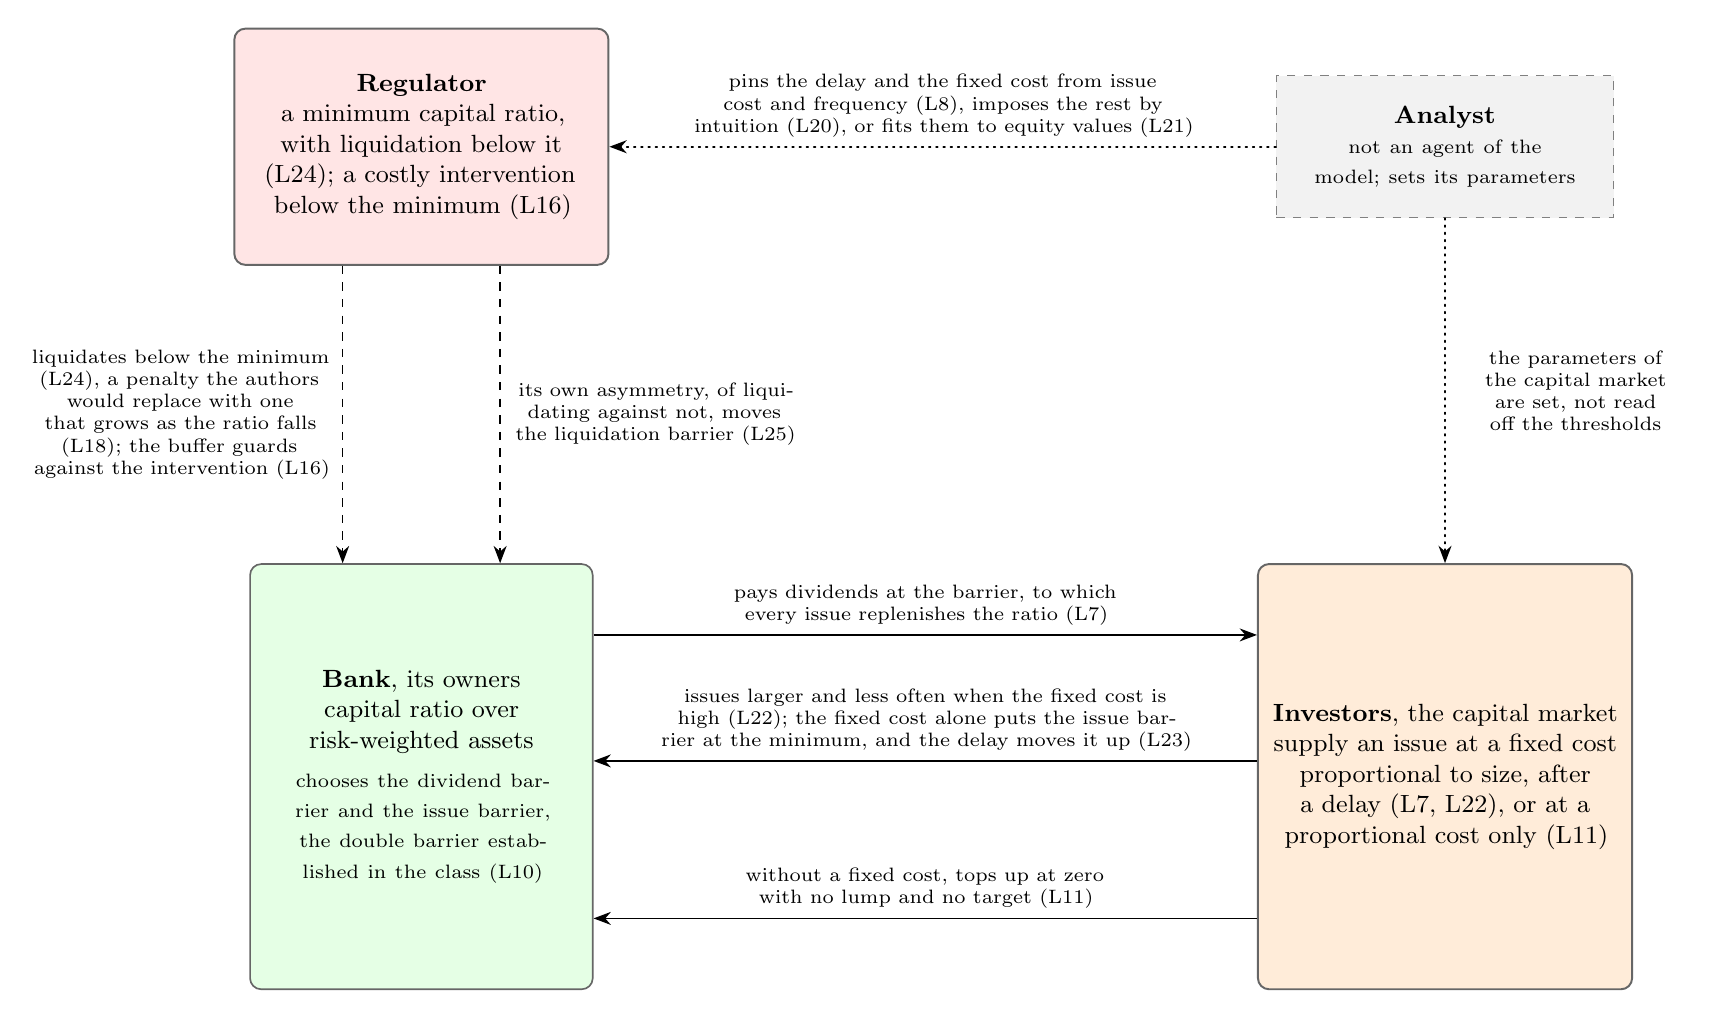
\begin{tikzpicture}[ledger]
\node[regulator] (Reg) at (0,8) {\textbf{Regulator}\\ a minimum capital ratio, with liquidation below it (L24); a costly intervention below the minimum (L16)};
\node[agent, minimum height=5.4cm] (Bank) at (0,0) {\textbf{Bank}, its owners\\ capital ratio over risk-weighted assets\\[3pt] \scriptsize chooses the dividend barrier and the issue barrier, the double barrier established in the class (L10)};
\node[other, minimum height=5.4cm] (Inv) at (13,0) {\textbf{Investors}, the capital market\\ supply an issue at a fixed cost proportional to size, after a delay (L7, L22), or at a proportional cost only (L11)};
\node[outside] (An) at (13,8) {\textbf{Analyst}\\ \scriptsize not an agent of the model; sets its parameters};

\draw[settled] ([yshift=18mm]Bank.east) -- node[lab, pos=0.5, above=2pt, text width=7.4cm] {pays dividends at the barrier, to which every issue replenishes the ratio (L7)} ([yshift=18mm]Inv.west);
\draw[settled] ([yshift=2mm]Inv.west) -- node[lab, pos=0.5, above=2pt, text width=7.4cm] {issues larger and less often when the fixed cost is high (L22); the fixed cost alone puts the issue barrier at the minimum, and the delay moves it up (L23)} ([yshift=2mm]Bank.east);
\draw[settled] ([yshift=-18mm]Inv.west) -- node[lab, pos=0.5, above=2pt, text width=7.4cm] {without a fixed cost, tops up at zero with no lump and no target (L11)} ([yshift=-18mm]Bank.east);
\draw[given]   ([xshift=-10mm]Reg.south) -- node[lab, pos=0.5, anchor=east, xshift=-3pt, text width=3.8cm] {liquidates below the minimum (L24), a penalty the authors would replace with one that grows as the ratio falls (L18); the buffer guards against the intervention (L16)} ([xshift=-10mm]Bank.north);
\draw[given]   ([xshift=10mm]Reg.south) -- node[lab, pos=0.5, anchor=west, xshift=3pt, text width=3.6cm] {its own asymmetry, of liquidating against not, moves the liquidation barrier (L25)} ([xshift=10mm]Bank.north);
\draw[open]    (An.west) -- node[lab, pos=0.5, above=2pt, text width=6.4cm] {pins the delay and the fixed cost from issue cost and frequency (L8), imposes the rest by intuition (L20), or fits them to equity values (L21)} (Reg.east);
\draw[open]    (An.south) -- node[lab, pos=0.5, anchor=west, xshift=3pt, text width=3.0cm] {the parameters of the capital market are set, not read off the thresholds} (Inv.north);
\end{tikzpicture}
}
\caption{Issuance-cost barrier models, \citet{peura2006},
\citet{daihuangkeppo2019}, \citet{bolton2011}, \citet{lokka2008} and
\citet{milnewhalley2001}. Solid arrows are derived in the papers and proved in
their Lean records, dashed arrows are assumed, and dotted arrows are stated in
words and not modelled. The analyst is not an agent of the models. Against
Figure~\ref{fig:ledger}, there is no cap and no graduated penalty, and the
parameters are set rather than read off the thresholds.}
\label{fig:ledger-issuance}
\end{figure}

\begin{figure}[p]
\centering
\adjustbox{max width=\linewidth, max height=0.80\textheight}{% ledger_cap.tex, Figure 3 of wealth_garch_theory.tex: regulatory-cap
% control, with Black and Perold's rule as the same geometry under
% preferences. Labels cite the literature rows.
\sffamily
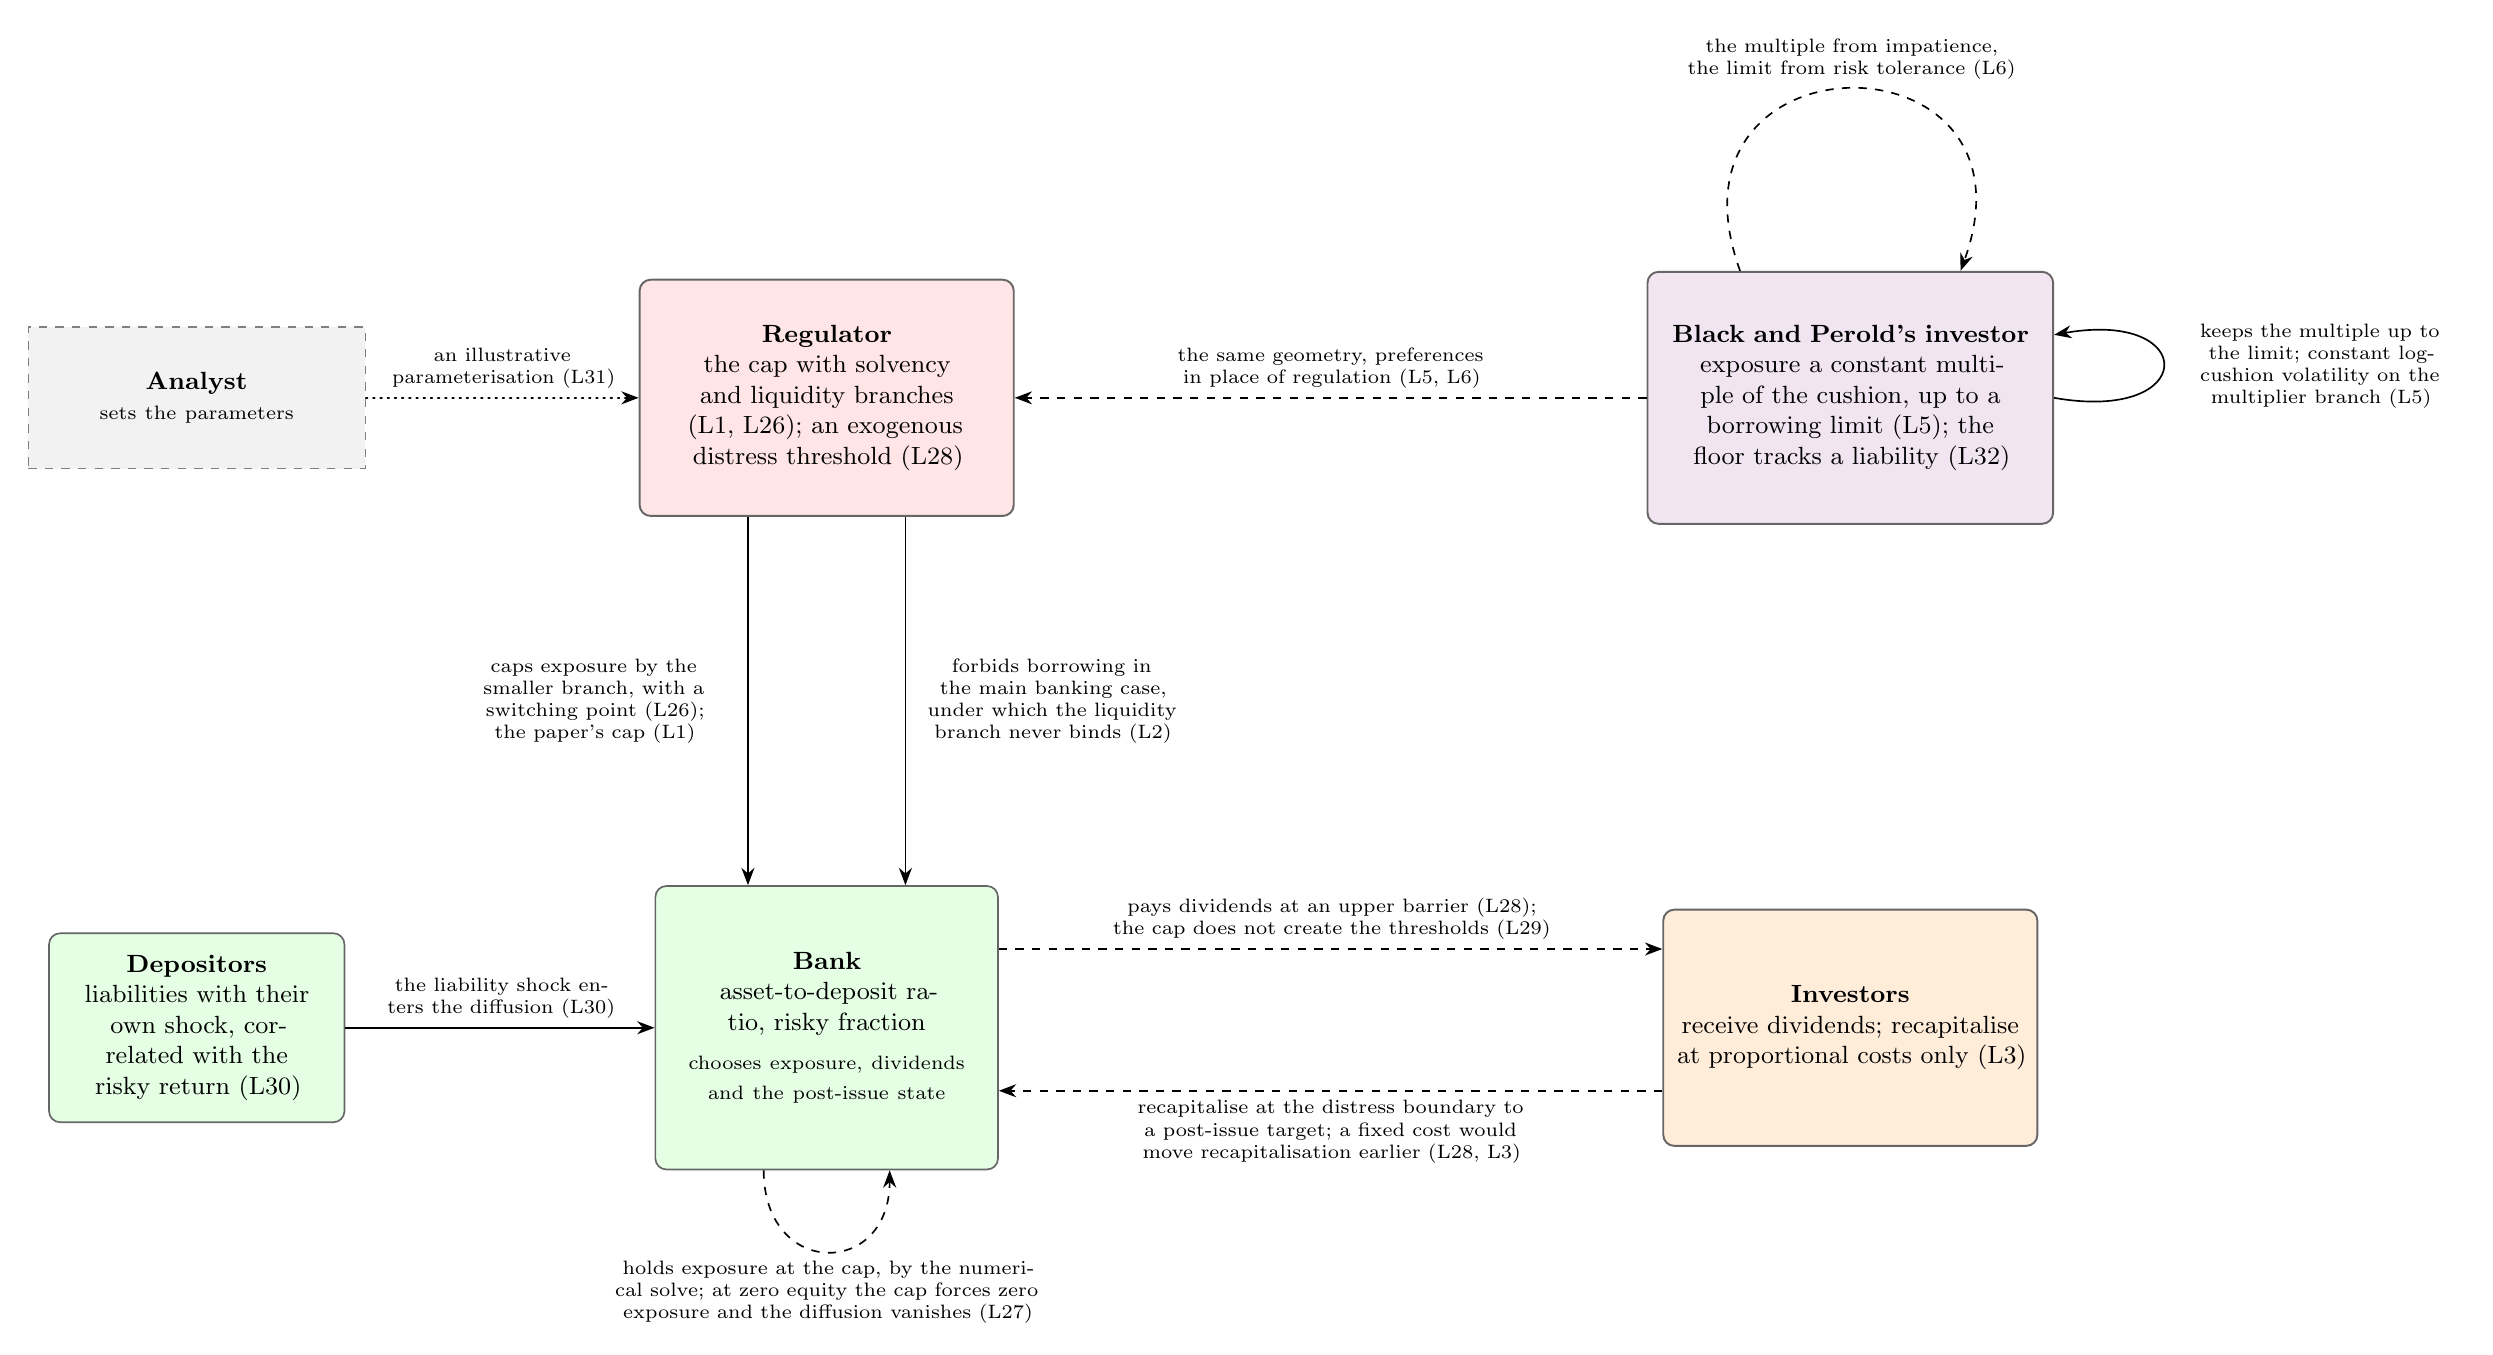
\begin{tikzpicture}[ledger]
\node[regulator] (Reg) at (0,8) {\textbf{Regulator}\\ the cap with solvency and liquidity branches (L1, L26); an exogenous distress threshold (L28)};
\node[agent, minimum height=3.6cm] (Bank) at (0,0) {\textbf{Bank}\\ asset-to-deposit ratio, risky fraction\\[3pt] \scriptsize chooses exposure, dividends and the post-issue state};
\node[other] (Inv) at (13,0) {\textbf{Investors}\\ receive dividends; recapitalise at proportional costs only (L3)};
\node[agent, text width=3.4cm, minimum height=2.4cm] (Dep) at (-8,0) {\textbf{Depositors}\\ liabilities with their own shock, correlated with the risky return (L30)};
\node[pref, text width=4.8cm, minimum height=3.2cm] (BP) at (13,8) {\textbf{Black and Perold's investor}\\ exposure a constant multiple of the cushion, up to a borrowing limit (L5); the floor tracks a liability (L32)};
\node[outside] (An) at (-8,8) {\textbf{Analyst}\\ \scriptsize sets the parameters};

\draw[settled] ([xshift=-10mm]Reg.south) -- node[lab, pos=0.5, anchor=east, xshift=-3pt, text width=3.6cm] {caps exposure by the smaller branch, with a switching point (L26); the paper's cap (L1)} ([xshift=-10mm]Bank.north);
\draw[settled] ([xshift=10mm]Reg.south) -- node[lab, pos=0.5, anchor=west, xshift=3pt, text width=3.4cm] {forbids borrowing in the main banking case, under which the liquidity branch never binds (L2)} ([xshift=10mm]Bank.north);
\draw[given]   ([xshift=-8mm]Bank.south) to[out=-90, in=-90, looseness=2.2] node[lab, pos=0.5, below=2pt, text width=6.4cm] {holds exposure at the cap, by the numerical solve; at zero equity the cap forces zero exposure and the diffusion vanishes (L27)} ([xshift=8mm]Bank.south);
\draw[given]   ([yshift=10mm]Bank.east) -- node[lab, pos=0.5, above=2pt, text width=7.2cm] {pays dividends at an upper barrier (L28); the cap does not create the thresholds (L29)} ([yshift=10mm]Inv.west);
\draw[given]   ([yshift=-8mm]Inv.west) -- node[lab, pos=0.5, below=2pt, text width=7.2cm] {recapitalise at the distress boundary to a post-issue target; a fixed cost would move recapitalisation earlier (L28, L3)} ([yshift=-8mm]Bank.east);
\draw[settled] (Dep.east) -- node[lab, pos=0.5, above=2pt, text width=3.0cm] {the liability shock enters the diffusion (L30)} (Bank.west);
\draw[settled] (BP.east) to[out=-10, in=10, looseness=6] node[lab, pos=0.5, anchor=west, xshift=4pt, text width=3.6cm] {keeps the multiple up to the limit; constant log-cushion volatility on the multiplier branch (L5)} ([yshift=8mm]BP.east);
\draw[given]   ([xshift=-14mm]BP.north) to[out=110, in=70, looseness=3] node[lab, pos=0.5, above=2pt, text width=4.6cm] {the multiple from impatience, the limit from risk tolerance (L6)} ([xshift=14mm]BP.north);
\draw[given]   (BP.west) -- node[lab, pos=0.5, above=2pt, text width=4.6cm] {the same geometry, preferences in place of regulation (L5, L6)} (Reg.east);
\draw[open]    (An.east) -- node[lab, pos=0.5, above=2pt, text width=2.8cm] {an illustrative parameterisation (L31)} (Reg.west);
\end{tikzpicture}
}
\caption{Regulatory-cap control, \citet{bayraktar2026}, with the rule of
\citet{blackperold1992} as the same geometry under preferences. Arrow styles as
in Figure~\ref{fig:ledger-issuance}. Against Figure~\ref{fig:ledger}, there is
no fixed issuance cost, the trigger is exogenous, and there is no asymmetry
parameter.}
\label{fig:ledger-cap}
\end{figure}

\begin{figure}[p]
\centering
\adjustbox{max width=\linewidth, max height=0.80\textheight}{% ledger_preference.tex, Figure 4 of wealth_garch_theory.tex: preference
% asymmetry read in volatility. No bank and no regulator. Labels cite the
% literature rows.
\sffamily
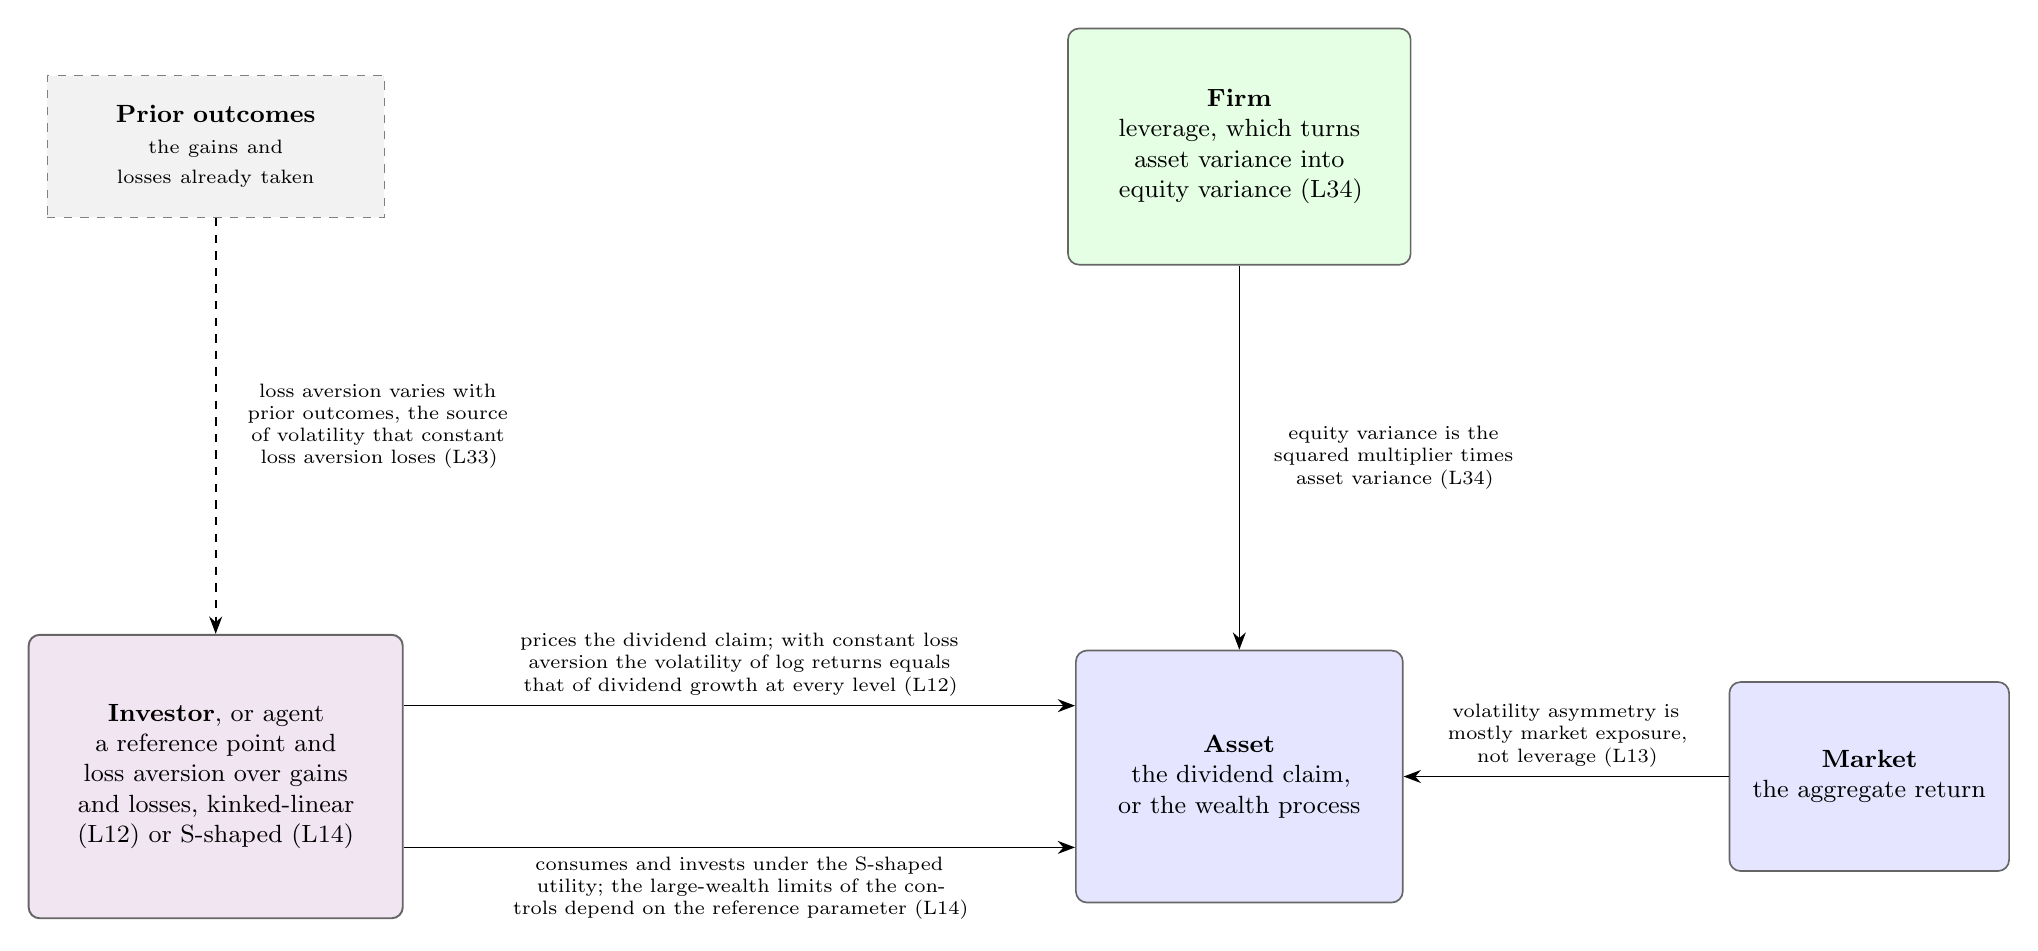
\begin{tikzpicture}[ledger]
\node[pref, minimum height=3.6cm] (Inv) at (0,0) {\textbf{Investor}, or agent\\ a reference point and loss aversion over gains and losses, kinked-linear (L12) or S-shaped (L14)};
\node[object, minimum height=3.2cm] (Asset) at (13,0) {\textbf{Asset}\\ the dividend claim, or the wealth process};
\node[agent] (Firm) at (13,8) {\textbf{Firm}\\ leverage, which turns asset variance into equity variance (L34)};
\node[outside] (Prior) at (0,8) {\textbf{Prior outcomes}\\ \scriptsize the gains and losses already taken};
\node[object, text width=3.2cm, minimum height=2.4cm] (Mkt) at (21,0) {\textbf{Market}\\ the aggregate return};

\draw[settled] ([yshift=9mm]Inv.east) -- node[lab, pos=0.5, above=2pt, text width=7.6cm] {prices the dividend claim; with constant loss aversion the volatility of log returns equals that of dividend growth at every level (L12)} ([yshift=9mm]Asset.west);
\draw[settled] ([yshift=-9mm]Inv.east) -- node[lab, pos=0.5, below=2pt, text width=7.6cm] {consumes and invests under the S-shaped utility; the large-wealth limits of the controls depend on the reference parameter (L14)} ([yshift=-9mm]Asset.west);
\draw[given]   (Prior.south) -- node[lab, pos=0.5, anchor=west, xshift=3pt, text width=3.8cm] {loss aversion varies with prior outcomes, the source of volatility that constant loss aversion loses (L33)} (Inv.north);
\draw[settled] (Firm.south) -- node[lab, pos=0.5, anchor=west, xshift=3pt, text width=3.6cm] {equity variance is the squared multiplier times asset variance (L34)} (Asset.north);
\draw[settled] (Mkt.west) -- node[lab, pos=0.5, above=2pt, text width=3.0cm] {volatility asymmetry is mostly market exposure, not leverage (L13)} (Asset.east);
\end{tikzpicture}
}
\caption{Preference asymmetry read in volatility, \citet{barberis2001},
\citet{li2023} and \citet{engle2018}. Arrow styles as in
Figure~\ref{fig:ledger-issuance}. There is no bank and no regulator. Against
Figure~\ref{fig:ledger}, the asymmetry is sought in the variance of returns,
which a binding cap closes (M11), and not in thresholds.}
\label{fig:ledger-preference}
\end{figure}
\end{landscape}

\subsection{The three approaches in one formulation}
\label{sec:common}

The paper's model, A1 to A6, holds the three approaches as restrictions of its
parameters, the asymmetry parameter $\lambda_S$, the fixed issuance cost $K$,
the proportional issuance cost $\kappa$, the regulatory cap $u$, and the
liability volatility $\sigma_L$ with the return-liability correlation $c$.
Table~\ref{tab:common} gives the restriction for each paper read, and
Table~\ref{tab:common-values} evaluates two quantities on each. One is the
determinant of the two thresholds in the two frictions $\theta_1,\theta_2$ that
an approach has,
\[
J=\det\frac{\partial(y^*,x_L)}{\partial(\theta_1,\theta_2)} ,
\]
read in the issuance-cost models with their dividend barrier and issue barrier
in place of the dividend barrier and the recapitalisation trigger. The other is
the pair of limits of buffer variance, $\nu_1^2$ and $\nu_3^2$, where the risky
exposure binds the cap. Each value is at the paper's own parameters, so the
comparison is of signs and of which quantity exists, rather than of sizes
across papers. The last column of Table~\ref{tab:common} names what the
formulation does not hold.

The determinant separates the paper from the issuance-cost models. In the
table of \citet{peura2006} the delay and the fixed cost give $J=-29/100$ at
small costs and $J=+1/25$ at the highest cost (L8, L41, L42, L43), so the two
frictions are separated at each point of the table by the size of their
responses and not by a sign that holds throughout it. In
\citet{daihuangkeppo2019} the delay and the fixed cost move the issue barrier the
same way and
$J\approx-0.0041$ (L9, L44), non-zero by magnitude. \citet{milnewhalley2001}
report like signs for the audit and the fixed cost and print no values (L40),
so $J$ cannot be formed. In the paper $J<0$ under the hypotheses of M1 to M3
by the signs of the responses alone (M3), so the separation does not rest on a
calibration.

The limits separate the paper from regulatory-cap control and from the
preference approach. At the baseline of \citet{bayraktar2026}, which they do
not evaluate, the deficit limit is about $3.140$ and the surplus limit about
$0.0688$, a ratio of about $45.6$ (M13, L45, L46), and without borrowing, their
main banking case, the surplus limit is not reached (C3). With no liability
shock the same limits are $256/81\approx3.160$ and $16/225\approx0.0711$, the
log-cushion variances of capped portfolio insurance with multiples $1/a_1$ and
$1/a_3$ (M14, L5), so at that baseline the unhedged liability shock lowers the
deficit limit by about $0.6$ percent and the surplus limit by about $3.2$
percent. The bank of \citet{daihuangkeppo2019} has no liability shock (L47),
and in the rule of \citet{blackperold1992} the safe asset can hedge it (L32)
and the multiples are set by preferences (L6). In the unconstrained control of
\citet{li2023} the large-wealth limits depend on the reference
parameter (L14), while in the paper neither limit depends on the asymmetry
parameter (M11). In \citet{barberis2001} constant loss aversion leaves the
volatility of returns at that of dividend growth, $12$ percent at every level
(L12), free of the asymmetry because the price-dividend ratio is constant
rather than because a cap binds.

\begin{table}[H]
\footnotesize
\caption{The three approaches as restrictions of the paper's model.}\label{tab:common}
\begin{tabular}{@{}P{2.8cm}P{2.9cm}P{2.4cm}P{1.9cm}P{2.1cm}P{2.7cm}@{}}
\toprule
Paper & Shortfall side & Issuance side & Regulatory cap & Recapitalisation trigger & Outside the formulation \\
\midrule
\citet{peura2006} & $\lambda_S=1$, liquidation at the minimum (L24) & $K>0$ (L7) & none & endogenous & the delay on issues (L23) \\ \addlinespace
\citet{daihuangkeppo2019} & $\lambda_S=1$, the regulator's asymmetry in liquidation (L25) & $K>0$ (L9) & none & endogenous & the delay, partial information \\ \addlinespace
\citet{milnewhalley2001} & $\lambda_S=1$, an audit at random below the minimum (L38) & $K>0$ (L39) & none & endogenous (L38) & the random audit \\ \addlinespace
\citet{bayraktar2026} & $\lambda_S=1$ & $K=0$, $\kappa>0$ (L3, L46) & $u$ (L26) & exogenous (L28) & none \\ \addlinespace
\citet{blackperold1992} & no asymmetry & no issuance & $u$ with $a_2=0$, slopes from preferences (L5, L6) & none & preferences over consumption \\ \addlinespace
\citet{barberis2001}, \citet{li2023} & loss aversion over gains and losses (L36, L14) & no issuance & none & none & not a bank \\ \addlinespace
This paper & $\lambda_S\ge1$, $R=1+q$ (A4) & $K>0$, $\kappa\ge0$ (A5) & $u$ (A2) & endogenous (A6) & none \\
\bottomrule
\end{tabular}
\end{table}

\begin{table}[H]
\footnotesize
\caption{The two quantities of the common formulation, each at the paper's own parameters.}\label{tab:common-values}
\begin{tabular}{@{}P{3.0cm}P{2.4cm}P{4.0cm}P{3.6cm}P{2.6cm}@{}}
\toprule
Paper & Two frictions & Determinant $J$ of the two thresholds & Limits of buffer variance & The asymmetry enters \\
\midrule
\citet{peura2006} & delay, fixed cost & $-29/100$ at small costs, $+1/25$ at the highest (L8, L41) & not evaluated & nowhere \\ \addlinespace
\citet{daihuangkeppo2019} & delay, fixed cost & about $-0.0041$, like signs (L44) & not evaluated & the liquidation barrier (L25) \\ \addlinespace
\citet{milnewhalley2001} & audit, fixed cost & like signs, no values (L40) & not evaluated & nowhere \\ \addlinespace
\citet{bayraktar2026} & one cost & none, the trigger is exogenous (L28) & about $3.140$ and $0.0688$ at their baseline (M13), the second not reached without borrowing (C3) & nowhere \\ \addlinespace
\citet{blackperold1992} & none & no trigger & $256/81$ and $16/225$ at the same slopes, with no liability shock (M14) & the slopes, by preferences (L6) \\ \addlinespace
\citet{barberis2001}, \citet{li2023} & none & no trigger & return volatility $12$ percent at every level (L12); limits that depend on the reference (L14) & the limits, without a cap (L14) \\ \addlinespace
This paper & $\lambda_S$, $K$ & $J<0$ by sign (M3) & free of $\lambda_S$ (M11) & the thresholds (M1 to M3) \\
\bottomrule
\end{tabular}
\end{table}

\subsection{Papers read}

\footnotesize
\begin{longtable}{@{}P{0.8cm}P{2.2cm}P{3.5cm}P{5.5cm}P{1.3cm}P{1.9cm}@{}}
\caption{Papers read, with the passage each row relies on.}\label{tab:literature}\\
\toprule
ID & Paper & What we rely on & Quote & Page & Rows \\
\midrule
\endfirsthead
\toprule
ID & Paper & What we rely on & Quote & Page & Rows \\
\midrule
\endhead
\lrow{L1}{bayraktar2026}{The cap $u$ and the crossing point $\bar x$ of M10 are this paper's eq.~(4) and its switching point. M10 and M11 are statements about its cap. The parallel ends there, since the paper evaluates no limit of the volatility and has no asymmetry parameter.}{the parameter a3 scales the entire liquidity constraint and determines its asymptotic upper bound}{17}{M10, M11}
\lrow{L2}{bayraktar2026}{The authors' main banking case has no borrowing. With no borrowing the liquidity branch lies above the ceiling once $a_2\le(1-a_3)x$, so it never binds (\lean{BCVW.ceiling_tighter_than_lcr}), and M11's surplus limit belongs to their unrestricted benchmark.}{we treat the π ≤ 1 case as the main banking interpretation and the unrestricted case as a mathematical benchmark}{19}{M11}
\lrow{L3}{bayraktar2026}{The paper has no fixed issuance cost, fixes its recapitalisation threshold exogenously, and names a fixed cost as a change that could move recapitalisation. M2 and M3 take up that change.}{If one introduced fixed issuance costs, endogenous market access, or adverse-selection costs that rise near distress, earlier recapitalization or inaction at the boundary could become optimal.}{13}{M2, M3}
\lrow{L4}{bayraktar2026}{A fixed issuance cost charged in dollars breaks the reduction to one dimension. M1 to M3 charge $K$ per unit of liabilities, which keeps it (Appendix~\ref{app:scope}).}{Fixed issuance costs, nonlinear issuance costs, taxes, deposit insurance premia, endogenous deposit rates, balance-sheet size effects, multiple asset classes, or regulatory constraints depending on dollar levels rather than ratios would generally break the one-dimensional reduction.}{9}{M1, M2, M3}
\lrow{L5}{blackperold1992}{Their rule is the regulatory cap with $a_2=0$, multiple $1/a_1$ and leverage limit $1/a_3$ (\lean{BlackPerold.cap_is_cppi}), and its log-cushion volatility on the multiplier branch is constant (their Prop.~2), the constancy of $\nu_1^2$ in M10. The parallel ends at the liability, which their reserve asset tracks and ours does not.}{maintains the portfolio's risk exposure a constant multiple of the excess of wealth over a floor, up to a borrowing limit}{403}{M10, M11}
\lrow{L6}{blackperold1992}{In their Prop.~11 the multiple is set by the impatience to consume and the leverage limit by risk aversion, so the two volatility levels carry preference information. In M11 the slopes are regulatory and the asymmetry parameter is absent from the limits.}{The multiple depends on the utility function only through}{421}{M11}
\lrow{L7}{peura2006}{The bank form of the class, with a fixed issuance cost as a fixed proportion of size, the device of M1 to M3, and each issue ending at the dividend barrier, a single target as in M7.}{As in the general case, the dividend barrier is also the level up to which the capital ratio is replenished each time a new capital issue is implemented.}{2176}{M1, M2, M7}
\lrow{L8}{peura2006}{They pin the issue delay and the fixed cost by calibration from issue cost and frequency, moments of the thresholds, and their Table 2 has the sign pattern of M3 in the delay and the fixed cost at small costs (\lean{PeuraKeppo.table2_det_neg}). The parallel ends at the parameter, a delay rather than a preference, and at the method, a calibration rather than a local identification theorem.}{For D and K, we identify common estimates across banks such that their implied capital raising cost and frequency are of plausible magnitude.}{2184}{M3}
\lrow{L9}{daihuangkeppo2019}{Their Table 2.1 gives the responses of the dividend and recapitalisation barriers to seven parameters, the fixed cost with the signs of M1 and M2 (\lean{DaiHuangKeppo.table21_K_signs}). They state no identification and have no shareholder asymmetry parameter, and their delay and fixed cost move the trigger the same way.}{K 0.0017 −0.0543 0 −0.0004}{76}{M1, M2, M3}
\lrow{L10}{bolton2011}{Its authors state that the double barrier of payout and external financing is an established structure. Its fixed issuance cost is proportional to capital to keep the model homogeneous, as in M1 to M3, and each issue returns to one target, as in M7.}{While this double-barrier policy is not new (it goes back to the inventory model of Miller and Orr 1966 in corporate finance), our model provides substantial new insight}{3}{M1, M7}
\lrow{L11}{lokka2008}{With proportional issuance costs only, issuance is a minimal reflection at zero, neither a lump nor a target. The fixed issuance cost is what produces the single target of M7.}{In this problem, it is optimal to issue minimal new equity so as to reflect the reserves process at 0 and make minimal dividend payments so as to reflect the reserves process at a certain level x∗ (see Section 4).}{2}{M7}
\lrow{L12}{barberis2001}{With a constant level of loss aversion, the volatility of log returns equals that of dividend growth for every level, the parallel to the absence of $\lambda_S$ from the limits of M11. The parallel ends at the mechanism, a constant price-dividend ratio in an endowment economy rather than a binding regulatory cap.}{the volatility of log returns in this model is equal to the volatility of log dividend growth, namely 12 percent.}{47}{M11}
\lrow{L13}{engle2018}{They split observed equity volatility asymmetry into a mechanical-leverage share and a market-exposure share. The parallel ends at the object, a response of variance to the sign of news rather than limits of variance across regions of a state variable.}{Volatility asymmetry is mostly explained by exposure to the aggregate market, not a mechanical leverage effect.}{449}{M11}
\lrow{L14}{li2023}{In an unconstrained loss-averse control the large-wealth limits of the optimal controls depend on the preference parameters, the contrast to M11, where a binding regulatory cap fixes them.}{our asymptotic limits differ significantly from the ones in the Merton's problem, which now sensitively depends on the reference degree parameter}{13}{M11}
\lrow{L15}{berger2008}{Buffers well above the minimum are the fact the shortfall penalty of A4 and M8 is to explain. The parallel ends at the method, a partial-adjustment regression without a model of the thresholds.}{Since the early 1990s, however, the largest U.S. banking organizations have maintained ratios well in excess of regulatory minimums.}{1}{M8}
\lrow{L16}{milnewhalley2001}{The buffer guards against the supervisor's intervention or the market's response below the minimum, the reading of the penalty in Appendix~\ref{app:scope}. Their cost is an audit at random times, not a graduated running penalty.}{What matters instead is the possibility of future capitalisation falling below minimum required levels and inducing a costly regulatory intervention or market response.}{3}{M8}
\lrow{L17}{peura2006}{The optimising bank with a fixed issuance cost (M6) and liquidation at the minimum underpredicts the capital level, on their own calibration. The shortfall penalty of A4, whose form M8 carries, is the friction added.}{The model falls somewhat short of explaining the level of capital held by banks.}{2188}{M6, M8}
\lrow{L18}{peura2006}{The graduated penalty they call for is $\Lambda$ of A4 and M8, with the asymmetry parameter $\lambda_S$ setting how much it charges. The parallel ends at the call, since they do not add it.}{A model in which the penalty gradually increases as the capital ratio deteriorates would therefore be more realistic.}{2192}{M8}
\lrow{L19}{peura2006}{The question they leave, whose cost binds the bank's capital. The thresholds identify the asymmetry parameter under any reading and do not choose among them.}{Whether these omissions matter reduces to the issue of which constituency provides the binding constraint on bank capitalization.}{2192}{M3, M8}
\lrow{L20}{peura2006}{Their parameters beyond the return moments are imposed, not identified from the bank's policy. M3 identifies two of them from the thresholds.}{imposed common values for other parameters (mainly guided by high level economic intuition)}{2192}{M3}
\lrow{L21}{daihuangkeppo2019}{Their parameters are fitted to equity values, not identified from the thresholds.}{are calibrated by fitting the partially observed value function}{84}{M3}
\lrow{L22}{peura2006}{Issues are larger and rarer when the fixed cost is high, the widening trigger-to-target gap of M2 and the finite count of M6.}{The owners optimally issue new equity in larger quantities but less frequently when the cost of issuance is high}{2179}{M2, M6}
\lrow{L23}{peura2006}{In their model the fixed cost alone puts the issue barrier at the minimum, and the delay moves it up. In M2 the trigger is an interior threshold whose responses to the fixed issuance cost and to the asymmetry parameter are derived.}{The sole presence of the fixed cost does not generate a positive capital issue barrier and will not result in a positive probability of liquidation.}{2177}{M2}
\lrow{L24}{peura2006}{The penalty at the minimum is liquidation. The shortfall penalty of M8 grades it below the reference.}{We assume that the corrective action from violation of the minimum capital requirement will be liquidation}{2168}{M8}
\lrow{L25}{daihuangkeppo2019}{The asymmetry in their model is the regulator's, between the costs of liquidating and of not liquidating, and it acts through the liquidation barrier. The asymmetry parameter of M2 and M3 is in the bank's objective and moves the trigger against the fixed issuance cost.}{when the liquidation parameter a rises, then the liquidation barrier I falls}{71}{M2, M3}
\lrow{L26}{bayraktar2026}{The minimum of two branches with a switching point, the cap and the crossing point of M10.}{The key structure is the minimum operator in the regulatory constraint, with a switching point}{15}{M10}
\lrow{L27}{bayraktar2026}{At zero equity the cap forces zero exposure and the diffusion vanishes, the boundary that M9 sends to minus infinity and near which M11 takes its deficit limit.}{At the hypothetical zero-equity level y = 1, the solvency constraint forces π = 0 and the diffusion coefficient of the ratio process vanishes.}{11}{M9, M11}
\lrow{L28}{bayraktar2026}{Their dividend barrier and post-issue target are the paper's. Their trigger is the exogenous distress boundary, where the trigger of M2 is interior and responds to the two parameters.}{dividends are paid at an upper barrier, while recapitalization, when optimal, is triggered at the distress boundary and jumps to a post-issuance target}{12}{M1, M2, M7}
\lrow{L29}{bayraktar2026}{The cap moves the thresholds and does not create them, as in M1 and M2, where the costs make the thresholds and the cap of M10 shapes the variance.}{The regulatory constraints do not create the threshold structure from scratch}{13}{M1, M2, M10}
\lrow{L30}{bayraktar2026}{The liability shock is correlated with the risky return, as in A1, and enters the variance of M10 to M12.}{c is their shock correlation}{13}{M10, M11, M12}
\lrow{L31}{bayraktar2026}{Their parameters are illustrative and none is read off the policy, where M3 reads two off the thresholds.}{These values constitute an illustrative parameterization rather than an empirical calibration}{13}{M3}
\lrow{L32}{blackperold1992}{Their safe asset can track the liability, so the liability is hedged. In M10 to M12 the liability shock enters buffer variance unhedged.}{'safe' may mean that it closely tracks a liability stream}{404}{M10, M11}
\lrow{L33}{barberis2001}{Volatility from loss aversion needs loss aversion to vary over time. In M11 a constant asymmetry parameter leaves no mark on the limits of buffer variance, for a different reason, the binding cap.}{The investor's risk aversion is then constant over time, and stock prices lose an important source of volatility.}{4}{M11}
\lrow{L34}{engle2018}{Equity variance is the squared leverage multiplier times asset variance, the structural relation behind the change of variable of M10.}{which is the exact relationship implied by structural models of credit}{459}{M10}
\lrow{L35}{bayraktar2026}{Without borrowing the liquidity branch does not bind in the range of parameters they solve. C3 gives the condition under which it does not bind at any state.}{the LCR constraint is nonbinding within the parameter range considered}{20}{M11, M12}
\lrow{L36}{barberis2001}{Their loss-averse preference is kinked-linear at the reference, the form of the shortfall penalty of M8. It values gains and losses on an asset, not a shortfall of a bank's capital below its requirement.}{This is a piecewise linear function, shown as the solid line in Figure I. It is kinked at the origin, where the gain equals zero.}{10}{M8}
\lrow{L37}{milnewhalley2001}{The cost of falling below the minimum, through the audit, and the fixed cost of issue are joint determinants of the buffer, the two frictions that the asymmetry parameter and the fixed issuance cost stand for in A4 and A5.}{desired bank capital holdings are a function of cash-flow uncertainty, franchise value, audit frequency, recapitalisation costs, and cost of equity relative to deposits}{9}{M2, M3}
\lrow{L38}{milnewhalley2001}{Both frictions in one bank give an issue point and a target, the counterparts of the recapitalisation trigger and the injection target of M2 and M7.}{The bank capital decision is then akin to an (s, S) inventory problem.}{9}{M2, M7}
\lrow{L39}{milnewhalley2001}{Result 12. A higher fixed cost of issue or more frequent audit raises desired capital.}{always results in an increase in desired capital}{23}{M2, M3}
\lrow{L40}{milnewhalley2001}{Result 12. More frequent audit moves the policy the same way as a higher fixed cost of issue, so the two frictions have like responses, the case in which the control of M3 shows the Jacobian can be singular.}{A shift in the same direction would be produced by an increase of q.}{23}{M3}
\lrow{L41}{peura2006}{At $(\Delta,K)=(0.5,1.00)$ the printed values, with L42 and L43, give a determinant of the dividend and issue barriers in the delay and the fixed cost of $+1/25$ (\lean{PeuraKeppo.table2_det_high_K}), against $-29/100$ at small costs (\lean{PeuraKeppo.table2_det_value}). The values are printed to one decimal.}{.5 1.00 .9 3.7 2.8 27 122}{2184}{M3}
\lrow{L42}{peura2006}{At the highest cost a longer delay lowers the issue barrier, so the delay and the fixed cost move it the same way there.}{1 1.00 .6 3.8 3.2 24 291}{2184}{M3}
\lrow{L43}{peura2006}{The cost step of the determinant at the highest cost.}{.5 .50 1.1 3.5 2.4 17 57}{2184}{M3}
\lrow{L44}{daihuangkeppo2019}{With L9, the elasticity determinant of the two barriers in the delay and the fixed cost is $-103549/25000000$, about $-0.0041$ (\lean{DaiHuangKeppo.table21_det_value}), non-zero by magnitude while the two move the issue barrier the same way.}{∆ 0.0808 −0.1444 0 −0.0146}{76}{M3}
\lrow{L45}{bayraktar2026}{The cap geometry of the baseline at which M13 evaluates the limits of buffer variance.}{The baseline regulatory parameters are (a1 , a2 , a3 ) = (0.045, 0.05, 0.30)}{13}{M13}
\lrow{L46}{bayraktar2026}{The asset volatility, the liability volatility and the return-liability correlation of the baseline of M13.}{r = 0.02, µ = 0.04, µL = 0.03, ρ = 0.12, γ = 0.02, together with σ = 0.08, σL = 0.03, c = 0.20, κ = 0.01, κ′ = 0.02}{13}{M13}
\lrow{L47}{daihuangkeppo2019}{Their bank has no liability shock, which in M10 to M12 enters the limits of buffer variance.}{We ignore debt volatility and debt financing}{26}{M10, M11}
\lrow{L48}{constantinides1978}{A running penalty that grows linearly below a level and a fixed and a proportional cost of each transfer in one objective, the pairing of A4 and A5 in cash management rather than in a bank. Their trigger and target below the level are the recapitalisation trigger and the injection target of M2 and M7.}{model with both fixed and proportional transactions costs and with linear holding and penalty costs}{620}{M2, M7, M8}
\lrow{L49}{constantinides1978}{Their comparative statics are confined to special cases, an approximation with no drift and vanishing discounting, where M1 and M2 hold under the hypotheses of Appendix~\ref{app:evidence}.}{In this section and under additional assumptions we explicitly solve for the policy parameters and perform a comparative statics analysis.}{630}{M1, M2}
\lrow{L50}{constantinides1978}{In that approximation the upper trigger rises in the penalty and in the fixed cost of raising cash, the signs of M1 for the dividend barrier. They state no direction for the lower trigger or the lower target.}{the policy parameter u is an increasing function}{631}{M1}
\lrow{L51}{langmenno2026}{Their cost of breaching the buffer requirement is a charge per unit of loans that is the same at every shortfall (\lean{LangMenno.stigma_flat_below}), and with it the bank holds capital exactly at the buffer requirement. The shortfall penalty of M8 grows with the shortfall (\lean{LangMenno.graduated_grows_below}).}{Banks do not maintain voluntary capital buffers above the CBR}{18}{M8}
\lrow{L52}{constantinides1978}{In their approximation the four thresholds pin the penalty and the fixed cost of raising cash once the holding cost is known (\lean{Constantinides.thresholds_pin_pK}), an identification the authors do not state. M3 identifies the asymmetry parameter and the fixed issuance cost from two thresholds without a holding cost.}{We next consider the case where costs are not symmetric and there are fixed as well as proportional transactions costs.}{631}{M3}
\lrow{L53}{behn2019}{Their cost of breaching the capital requirement is a charge that does not grow with the shortfall (\lean{BehnEtAl.breach_flat_below}), the step the shortfall penalty of M8 grades.}{These costs are reminiscent of the bankruptcy cost in classical trade-off theory models}{10}{M8}
\lrow{L54}{behn2019}{They estimate the breach charge and an issuance cost with no fixed part (\lean{BehnEtAl.issueCost_no_fixed_part}) in one bank, and separate the two by the moments each is matched to rather than by the thresholds of the policy, as M3 does.}{The costs of breaching the minimum capital and liquidity requirements are mainly identified by the extent of the observed voluntary buffers}{23}{M3}
\lrow{L55}{glover2023}{A breach forces an issue priced at the proportional issuance cost, so one parameter charges both the shortfall and the issue (\lean{GloverEtAl.breach_slope_is_issuance_cost}) and no policy can separate them. M3 has two parameters, the asymmetry parameter and the fixed issuance cost.}{whenever the bank decides (or is forced) to raise new equity it will incur a cost}{10}{M3, M8}
\lrow{L56}{lambertini2014}{The capital requirement is a smooth log penalty on net worth, negative below required capital and a reward above it (\lean{LambertiniUysal.logTerm_pos_above}), with no kink. The shortfall penalty of M8 is zero at and above the reference and kinked there.}{Due to the log term, the bank is penalized when its capital goes below the required 8 percent of total assets}{23}{M8}
\lrow{L57}{decamps2011}{A fixed cost of each issue makes issues lumpy (\lean{DecampsEtAl.unitCost_falls}), the single target of M7.}{Because issuing shares involves a fixed cost, equity adjustments take place in lumpy and infrequent issues}{1503}{M7}
\lrow{L58}{alvarez2014}{In a fixed-cost inaction model the parameters are identified globally from moments of the distribution of adjustments rather than from thresholds, and two parameters that both raise kurtosis are separated only by adding the observed cost of adjustment (\lean{AlvarezLeBihanLippi.control_same_direction_not_identified}). M3 identifies two parameters from two thresholds by the opposite signs of their effects on one of them.}{the kurtosis of the price changes would not change. Moreover, kurtosis is increasing in both n and}{24}{M3}
\bottomrule
\end{longtable}
\normalsize

Every paper the tables name has been read in full and has a record with Lean
under \path{lit/}.

\section{What the paper adds to the three approaches}
\label{sec:novelty}

This section sets each theoretical result of the paper against the three
approaches of Section~\ref{sec:approaches}, and says what the result adds that
none of them has and what it shares with them. The comparison is with the
papers read in full, rather than with the literature at large. The claim
that K1 is new is concluded against those papers (C4), and the claim that K2
is new waits on what Table~\ref{tab:pending} names (C5).

The identification of K1 adds a second friction to the issuance-cost models
and a theorem to their tables. The responses of the dividend barrier and the
recapitalisation trigger to the fixed issuance cost are tabulated there (L9,
L22), and in the table of \citet{peura2006} the issue delay and the fixed
issuance cost move the trigger in opposite directions at small costs, with
both set by calibration to issue cost and frequency (L8). The paper's second
parameter is the asymmetry parameter of the graduated shortfall penalty that
Section~\ref{sec:literature} traces (L18, L24), rather than a delay. The responses of the two thresholds
to the asymmetry parameter and to the fixed issuance cost are derived under the
hypotheses of Appendix~\ref{app:evidence} (M1, M2) rather than read off a
solved case, and the opposite effect of the two parameters on the trigger gives
their local identification from the two thresholds (M3), where the papers read
set their parameters (L8, L20, L21). Regulatory-cap control has an exogenous trigger and no asymmetry
parameter (L28), and the preference approach has no trigger. K1 would be in
print if a paper read derived the responses of the thresholds to the asymmetry parameter of a
shortfall penalty in a bank's objective, and none of the three approaches has
such a parameter in a bank's objective (L12, L24, L28).

The limits of buffer variance in K2 add what regulatory-cap control leaves out. The
regulatory cap with its two branches is that of \citet{bayraktar2026} (L1,
L26), and the constant buffer variance on the solvency branch is the constant
log-cushion volatility of capped portfolio insurance (L5), so neither is
claimed new. The deficit limit and the surplus limit where the exposure binds
the cap, and the bound for every exposure within it (M11, M12), are not
evaluated by \citet{bayraktar2026} (L1). That the limits do not carry the
asymmetry parameter (M11) sets them apart from the two papers read in which
limits of a volatility carry a preference (L6, L14), as
Section~\ref{sec:literature} sets out, and the liability shock enters them
unhedged, where the safe asset of \citet{blackperold1992} can hedge it (L32). K2 would be in
print if a paper read evaluated the limits of buffer variance under a regulatory cap
with an unhedged liability shock, and none of the three approaches does. That the optimal
exposure binds the cap near both ends is a hypothesis of M11, and it is part of
what C5 waits on.

K1 and K2 together place the asymmetry parameter in the thresholds and not in
the limits of buffer variance, on one bank. The preference approach looks for the mark of
an asymmetry in the variance of returns, and finds none when the asymmetry is
constant (L12), while the issuance-cost models have thresholds and no
asymmetry parameter in the bank's objective (L24). Under the paper's regulatory
cap the limits of buffer variance carry nothing about the asymmetry parameter (M11) and
the two thresholds identify it (M3), so the paper reads the asymmetry
parameter off the thresholds, where the preference approach reads an asymmetry
off the variance of returns.

C3 replaces a range of parameters by a condition. \citet{bayraktar2026} find
that without borrowing the liquidity branch does not bind in the range they
solve (L2, L35), and C3 states that it does not bind at any state where
$a_2\le(1-a_3)x$, so that the surplus limit of M11 belongs to the leveraged
case.

The rest of the rows are shared with the issuance-cost models or are steps of
the argument, and the paper does not claim them new. The pair of a dividend
barrier and a recapitalisation trigger is an established double barrier (L10),
each issue returns
to one target as in \citet{peura2006} and \citet{bolton2011} (L7, L10), which
is M7, and a proportional cost alone gives no target (L11). The kinked-linear
form of the shortfall penalty is that of the loss-averse preference of
\citet{barberis2001} (L36), there over gains and losses on an asset and here
over a shortfall of equity below required capital (M8). The absence of a kink at
the recapitalisation trigger and the convexity just above it (M5, M4), the
finite number of issues (M6) and the capital buffer as a coordinate (M9) are
steps that the derivations of M1 to M3 and M10 to M12 use.

\section{Conclusions}
\label{sec:conclusions}

Table~\ref{tab:concl} holds the conclusions that rest on model rows and on
papers read in full. K1 rests on M1 to M4 and gives C1, C4 and C6. K2 rests
on M3 and M10 to M12 and gives C2 and C3, with C5 pending.
Table~\ref{tab:pending} holds every claim still waiting, and each of its rows
names what it waits on.

\footnotesize
\begin{longtable}{@{}P{0.8cm}P{12.3cm}P{3.4cm}@{}}
\caption{Conclusions resting on model rows and papers read.}\label{tab:concl}\\
\toprule
ID & Statement & Rows \\
\midrule
\endfirsthead
\toprule
ID & Statement & Rows \\
\midrule
\endhead
\crow{C1}{Under the hypotheses of Appendix~\ref{app:evidence}, the asymmetry parameter $\lambda_S$ and the fixed issuance cost $K$ are locally identified from the dividend barrier and the recapitalisation trigger. Both parameters raise the barrier, and they move the trigger in opposite directions, so the Jacobian of the two thresholds is non-singular.}{M1, M2, M3, M4}
\crow{C2}{Wherever the optimal exposure binds the cap near both ends, the limits of buffer variance are $\nu_1^2$ and $\nu_3^2$, functions of $(\sigma,\sigma_L,c,a_1,a_3)$ only, and for every compliant exposure buffer variance is bounded by $\max\{\sigma_L^2,\nu_1^2\}$. The asymmetry parameter moves the thresholds (C1) and is absent from these limits and bounds. In capped portfolio insurance, whose geometry the cap shares, the slopes come from preferences, so the same limits would carry them.}{M3, M10, M11, M12, L5, L6}
\crow{C3}{The surplus limit $\nu_3^2$ requires the liquidity branch to bind deep in surplus, which requires borrowing to hold the risky asset. With no borrowing, the main banking case of \citet{bayraktar2026}, the liquidity branch never binds once $a_2\le(1-a_3)x$, so the deficit limit and the bound of M12 are the results that apply there.}{M11, M12, L2}
\crow{C4}{In a bank's objective, the joint local identification of C1, of a shareholder asymmetry parameter of a shortfall penalty and a fixed issuance cost from the dividend barrier and the recapitalisation trigger by the opposite signs of their effects on the trigger, is new against the papers read in full. Its numerical precedents in other parameters are \citet{peura2006} and \citet{daihuangkeppo2019} (L8, L9). Outside banking, in the approximation of \citet{constantinides1978}, four thresholds pin a linear penalty and a fixed cost once a holding cost is known, a step the authors do not take (L52), and \citet{alvarez2014} identify a fixed-cost inaction model from moments of the distribution of adjustments rather than from thresholds, where two parameters that move one moment the same way need a second moment (L58).}{M3, L8, L9, L52, L58}
\crow{C6}{C1 supplies what the specification \citet{peura2006} call for (L18) lacks in their calibration. The asymmetry parameter and the fixed issuance cost are set by the two thresholds (M3) rather than imposed (L20) or fitted to equity values (L21). Which constituency the shortfall penalty stands for (L19) is not settled by the thresholds (Appendix~\ref{app:scope}).}{M3, L18, L19, L20, L21}
\bottomrule
\end{longtable}

\begin{longtable}{@{}P{0.8cm}P{12.3cm}P{3.4cm}@{}}
\caption{Claims not yet verified, each naming what it waits on.}\label{tab:pending}\\
\toprule
ID & Statement & Rows \\
\midrule
\endfirsthead
\toprule
ID & Statement & Rows \\
\midrule
\endhead
\crow{C5}{That under a regulatory two-branch cap with an unhedged liability shock the limits of buffer variance carry no information about the asymmetry parameter, while the thresholds do (C2), is new. \pend{Choulli, Taksar and Zhou (2003), SIAM J. Control Optim. 41(6), read in full with a record; and a proof that the optimal exposure binds the cap near both ends, the hypothesis of M11.}}{M11, L5, L6}
\bottomrule
\end{longtable}
\normalsize

\bibliographystyle{plainnat}
\bibliography{refs}

\appendix

\section{Proofs}
\label{app:proofs}

\paragraph{Notation.} The state is the assets-to-liabilities ratio
$x\in(1,\infty)$, $q>0$ required capital as a ratio, and
$z(x)=\log\big((x-1)/q\big)$ the capital buffer. The risky exposure is $\pi(x)$,
and the regulatory cap gives the capped exposure
$u(x)=\min\{(x-1)/a_1,(x-a_2)/a_3\}$ with crossing point
$\bar x=(a_3-a_1a_2)/(a_3-a_1)$. The diffusion of $x$ is
$\sigma^2(x,\pi)=\pi^2\sigma^2x^2+2\pi c\sigma\sigma_Lx(1-x)+\sigma_L^2(1-x)^2$,
with $\sigma$ the asset volatility, $\sigma_L$ the liability volatility and $c$
the return-liability correlation. Buffer variance is
$\zeta(x)=z'(x)^2\,\sigma^2\big(x,\pi(x)\big)$, the exposure ratio is
$\omega(x)=\pi(x)\,x/(x-1)$, and
$\nu_i^2=\sigma^2/a_i^2-2c\sigma\sigma_L/a_i+\sigma_L^2$ for $i\in\{1,3\}$.
$V$ is the value function, $y^*$ the dividend barrier, $x_L$ the
recapitalisation trigger and $y_{\text{post}}$ the injection target. $W$ is the
expected discounted shortfall and $N$ the discounted injection count under the
optimal policy, $\theta$ is $\lambda_S$ or $K$, and $F$ is $W$ or $N$
accordingly. $\rho_L$ is the liability-net discount rate, $\mu$ the drift of
$x$ along the cap and $\mu'$ its derivative in $x$, $\Lambda$ the shortfall
penalty and $R$ its reference, and $\ell=(R-x)^+$ for $F=W$ and $\ell=0$ for
$F=N$. Primes are derivatives in $x$. $\kappa$ is the proportional issuance
cost, $\mathcal MV$ the impulse operator, affine with slope $1+\kappa$ on the
intervention side, and $\mu=\mu(x_L)$ in M4 and M5. In M6, $e_i$ are the
discounted impulse times, $c_i$ the impulse terms and $B$ the cost bound.

\begin{mproof}{M1}{Identification.vppp_at_barrier, Identification.fpp_at_barrier, Identification.barrier_slope, Identification.barrier_slope_pos, Identification.control_barrier_sign_needs_gap, Envelope.wode_of_envelope, Envelope.node_of_envelope, Envelope.neumann_at_ystar}
\[ \tfrac12\sigma^2V'''+\tfrac12(\sigma^2)'V''+\mu V''+\mu'V'-\rho_LV'-\Lambda'=0,\quad V''=0,\ V'=1,\ \Lambda'=0\ \Rightarrow\ \tfrac12\sigma^2V'''=\rho_L-\mu' . \]
\[ \tfrac12\sigma^2F''+\mu F'-\rho_LF+\ell=0,\quad F'(y^*)=0,\ \ell(y^*)=0\ \Rightarrow\ \tfrac12\sigma^2F''=\rho_LF . \]
\[ V'''\frac{dy^*}{d\theta}+\partial_\theta V''=0,\quad \partial_\theta V''=-F''\ \Rightarrow\ \frac{dy^*}{d\theta}=\frac{F''}{V'''}=\frac{\rho_LF(y^*)}{\rho_L-\mu'(y^*)} . \]
Control, $\rho_L=1$, $\mu'=2$, $F=1$ $\Rightarrow$ $dy^*/d\theta=-1$.
\end{mproof}

\begin{mproof}{M2}{Identification.boundary_slope, Identification.trigger_rises_in_lambda, Identification.trigger_falls_in_K, Identification.target_rises_in_K, Identification.gap_increasing_in_K, Identification.control_trigger_slope_needs_curvature, Envelope.trigger_jump}
\[ V''(x)\frac{dx}{d\theta}+\partial_\theta V'(x)=0,\quad \partial_\theta V'=-F'\ \Rightarrow\ \frac{dx}{d\theta}=\frac{F'(x)}{V''(x)} . \]
\[ \frac{dx_L}{d\lambda_S}=\frac{W'(x_L)}{V''(x_L)}>0,\qquad \frac{dx_L}{dK}=\frac{N'(x_L)}{V''(x_L)}<0,\qquad \frac{dy_{\text{post}}}{dK}=\frac{N'(y_{\text{post}})}{V''(y_{\text{post}})}>0 . \]
\[ \frac{d(y_{\text{post}}-x_L)}{dK}>0,\qquad N(x_L)=N(y_{\text{post}})+1 . \]
Control, $V''(x)=0$, $F'(x)=0$ $\Rightarrow$ $dx=0$ and $dx=1$ both solve the chain rule.
\end{mproof}

\begin{mproof}{M3}{Identification.det_formula, Identification.det_neg_of_opposite, Identification.det_neg, Identification.control_same_direction_can_fail}
\[ \det\begin{pmatrix}\frac{\rho_LW(y^*)}{\rho_L-\mu'}&\frac{\rho_LN(y^*)}{\rho_L-\mu'}\\[2pt] \frac{W'(x_L)}{V''(x_L)}&\frac{N'(x_L)}{V''(x_L)}\end{pmatrix}=\frac{\rho_L}{(\rho_L-\mu')V''(x_L)}\big(W(y^*)N'(x_L)-N(y^*)W'(x_L)\big) . \]
\[ a_{11},a_{12},a_{21}>0>a_{22}\ \Rightarrow\ a_{11}a_{22}<0<a_{12}a_{21}\ \Rightarrow\ a_{11}a_{22}-a_{12}a_{21}<0 . \]
Control, $a_{11}=a_{12}=a_{21}=a_{22}=1$ $\Rightarrow$ $\det=0$.
\end{mproof}

\begin{mproof}{M4}{SecondOrder.psi_identity, SecondOrder.psi_nonneg_of_qvi, SecondOrder.trigger_convex, SecondOrder.trigger_strict_iff, SecondOrder.control_trigger_flat_when_psi_zero}
\[ \tfrac12\sigma^2V''+\mu V'-\rho_LV-\Lambda=0,\quad V'=1+\kappa\ \Rightarrow\ \tfrac12\sigma^2V''(x_L^+)=\rho_LV+\Lambda-(1+\kappa)\mu=\Psi(x_L) . \]
\[ \mu(1+\kappa)-\rho_LV-\Lambda\le0\ \Rightarrow\ \Psi(x_L)\ge0\ \Rightarrow\ V''(x_L^+)\ge0,\qquad \sigma^2>0\ \Rightarrow\ \big(V''(x_L^+)>0\iff\Psi(x_L)>0\big) . \]
Control, $\sigma^2=1$, $V'=1$, $\kappa=0$, $V=\Lambda=\mu=0$, $\rho_L=1$ $\Rightarrow$ $\Psi=0$, $V''(x_L^+)=0$.
\end{mproof}

\begin{mproof}{M5}{SmoothFit.hasDeriv_Mv, SmoothFit.kink_is_convex, SmoothFit.no_convex_kink, SmoothFit.smooth_fit, SmoothFit.control_kink_needs_obstacle, Envelope.smf_permits}
\[ V\ge\mathcal MV,\ \ V(x_L)=\mathcal MV(x_L),\ \ (\mathcal MV)'=1+\kappa\ \Rightarrow\ V'(x_L^+)\ge1+\kappa . \]
\[ V'(x_L^+)>1+\kappa\ \Rightarrow\ \tfrac12\sigma^2q+(1+\kappa)\mu-\rho_LV-\Lambda\le0\ \ \forall q,\qquad q=\frac{2(\rho_LV+\Lambda-(1+\kappa)\mu+1)}{\sigma^2}\ \Rightarrow\ 1\le0 . \]
\[ \Rightarrow\ V'(x_L^+)=1+\kappa;\qquad q\le0,\ \ (1+\kappa)\mu\le\rho_LV+\Lambda\ \Rightarrow\ \tfrac12\sigma^2q+(1+\kappa)\mu-\rho_LV-\Lambda\le0 . \]
Control, $v(x)=x$, $\kappa=1$, $\mathcal Mv(x)=2x$ $\Rightarrow$ $v(0)=\mathcal Mv(0)$, $v'(0^+)=1<2$.
\end{mproof}

\begin{mproof}{M6}{ImpulseCount.partial_sums_bounded, ImpulseCount.count_summable, ImpulseCount.count_le, ImpulseCount.impulse_sum_summable, ImpulseCount.control_count_needs_fixed_cost}
\[ K\sum_{i<n}e_i\le B,\ K>0\ \Rightarrow\ \sum_{i<n}e_i\le\frac BK\ \ \forall n,\qquad e_i\ge0\ \Rightarrow\ N=\sum_ie_i\le\frac BK<\infty . \]
\[ |c_i|\le Ce_i\ \Rightarrow\ \sum_i|c_i|\le C\,N<\infty . \]
Control, $K=0$, $e_i=1$ $\Rightarrow$ $0\le0$ for every $n$ and $\sum_ie_i=\infty$.
\end{mproof}

\begin{mproof}{M7}{Targeting.target_free_of_start, Targeting.target_same_for_all_starts, Targeting.control_target_moves_with_convex_cost}
\[ V(z)-(1+\kappa)(z-x)-K=\big(V(z)-(1+\kappa)z\big)+\big((1+\kappa)x-K\big), \]
\[ \arg\max_z\big(V(z)-(1+\kappa)(z-x)-K\big)=\arg\max_z\big(V(z)-(1+\kappa)z\big)\quad\forall x . \]
Control, $V(z)=2z$, cost $(z-x)^2$ $\Rightarrow$ $\arg\max_z\big(2z-(z-x)^2\big)=x+1$.
\end{mproof}

\begin{mproof}{M8}{QVI_Part1.lambda_asymmetry_vanishes_at_one, QVI_Part1.neg_Lambda_concave, QVI_Part1.control_concavity_needs_lambda_ge_one}
\[ \Lambda(x)\big|_{\lambda_S=1}=(1-1)(R-x)^+=0 . \]
\[ -\Lambda(x)=(\lambda_S-1)\big(\min\{x,R\}-R\big),\qquad \lambda_S-1\ge0,\ \ x\mapsto\min\{x,R\}\ \text{concave} . \]
Control, $\lambda_S=0$, $R=0$ $\Rightarrow$ $-\Lambda(x)=\max\{-x,0\}$, $-\Lambda(0)=0<\tfrac12=\tfrac12(-\Lambda(-1))+\tfrac12(-\Lambda(1))$.
\end{mproof}

\begin{mproof}{M9}{CapGeometry.zmap_inverse, CapGeometry.zmap_of_inverse, Coordinate.zmap_strictMonoOn, Coordinate.zmap_at_requirement, Coordinate.zmap_tendsto_atBot, Coordinate.zmap_tendsto_atTop}
\[ z(x)=\log\frac{x-1}{q},\qquad 1+qe^{z(x)}=x\ \ (x>1),\qquad z(1+qe^{w})=w . \]
\[ 1<x<y\ \Rightarrow\ \frac{x-1}{q}<\frac{y-1}{q}\ \Rightarrow\ z(x)<z(y),\qquad z(1+q)=\log1=0 . \]
\[ \frac{x-1}{q}\to0^+\ (x\to1^+)\ \Rightarrow\ z\to-\infty,\qquad \frac{x-1}{q}\to\infty\ (x\to\infty)\ \Rightarrow\ z\to\infty . \]
\end{mproof}

\begin{mproof}{M10}{CapGeometry.hasDerivAt_zmap, CapGeometry.zvol2_eq, CapGeometry.xbar_sub_one, CapGeometry.one_lt_xbar, CapGeometry.solvency_binds, CapGeometry.liquidity_binds, CapGeometry.zvol2_solvency}
\[ \frac{x-1}{a_1}\le\frac{x-a_2}{a_3}\iff(a_3-a_1)\,x\le a_3-a_1a_2\iff x\le\bar x,\qquad \bar x-1=\frac{a_1(1-a_2)}{a_3-a_1}>0 . \]
\[ z'(x)=\frac{1}{x-1},\qquad \zeta(x)=\omega(x)^2\sigma^2-2\,\omega(x)\,c\,\sigma\sigma_L+\sigma_L^2 . \]
\[ 1<x\le\bar x,\ \pi(x)\,x=u(x)\ \Rightarrow\ \omega(x)=\frac{1}{a_1}\ \Rightarrow\ \zeta(x)=\nu_1^2. \]
\end{mproof}

\begin{mproof}{M11}{CapGeometry.deficit_limit, CapGeometry.surplus_limit, CapGeometry.variance_ratio_is_cap_geometry, CapGeometry.control_surplus_limit_needs_a1_lt_a3, CapGeometry.control_constancy_needs_binding}
Near $1^+$, $\bar x>1$ by M10, so $1<x<\bar x$ eventually and $\zeta(x)=\nu_1^2$ there.
For $x\ge\bar x$,
\[ \omega(x)=\frac{x-a_2}{a_3(x-1)}=\frac{1}{a_3}+\frac{1-a_2}{a_3}\,(x-1)^{-1}\to\frac{1}{a_3}, \]
\[ \zeta(x)=\omega(x)^2\sigma^2-2\,\omega(x)\,c\,\sigma\sigma_L+\sigma_L^2\to\nu_3^2 . \]
Controls, at $\sigma=1$, $\sigma_L=c=0$, $q=1$.
\[ a_1=\tfrac12,\ a_2=0,\ a_3=\tfrac14\ \Rightarrow\ u(x)=2(x-1),\ \zeta\equiv4\ne16=\nu_3^2. \]
\[ \pi\equiv0\ \Rightarrow\ \zeta(2)=0\ne4=\nu_1^2. \]
\end{mproof}

\begin{mproof}{M12}{Bounds.qv_le_max, Bounds.zvol2_eq_qv, Bounds.nu2_eq_qv, Bounds.qv_zero, Bounds.deficit_bound, Bounds.surplus_bound, Bounds.control_bound_needs_long_exposure, Bounds.control_bound_needs_compliance}
\[ \zeta(x)=Q(\omega),\qquad Q(\omega)=\omega^2\sigma^2-2\omega c\sigma\sigma_L+\sigma_L^2,\qquad \omega=\frac{\pi(x)\,x}{x-1}, \]
\[ Q(0)=\sigma_L^2,\qquad Q(1/a_i)=\nu_i^2 . \]
\[ \omega=tM,\ t\in[0,1]\ \Rightarrow\ Q(\omega)=(1-t)Q(0)+tQ(M)+\sigma^2M^2(t^2-t)\le\max\{Q(0),Q(M)\} . \]
\[ 0\le\pi,\ \ \pi x\le u(x)\le\frac{x-1}{a_1}\ \Rightarrow\ 0\le\omega\le\frac1{a_1}\ \Rightarrow\ \zeta(x)\le\max\{\sigma_L^2,\nu_1^2\} . \]
\[ \pi x\le\frac{x-a_2}{a_3}\ \Rightarrow\ \omega\le w(x)=\frac1{a_3}+\frac{1-a_2}{a_3(x-1)}\to\frac1{a_3},\qquad Q(w(x))\to\nu_3^2 . \]
Controls, $(\sigma,\sigma_L,c)=(1,1,1)$, $\omega=-1$ $\Rightarrow$ $Q=4>1=\max\{Q(0),Q(1)\}$; $(\sigma,\sigma_L,c)=(1,0,0)$, $\omega=2>1$ $\Rightarrow$ $Q=4>1$.
\end{mproof}

\begin{mproof}{M13}{Comparison.nu1_baseline, Comparison.nu3_baseline, Comparison.ratio_baseline}
\[ \nu_1^2=\frac{0.08^2}{0.045^2}-\frac{2(0.20)(0.08)(0.03)}{0.045}+0.03^2=\frac{256}{81}-\frac{16}{750}+\frac{9}{10000}=\frac{2543449}{810000} . \]
\[ \nu_3^2=\frac{0.08^2}{0.30^2}-\frac{2(0.20)(0.08)(0.03)}{0.30}+0.03^2=\frac{16}{225}-\frac{4}{1250}+\frac{9}{10000}=\frac{6193}{90000} . \]
\[ \frac{\nu_1^2}{\nu_3^2}=\frac{2543449}{810000}\cdot\frac{90000}{6193}=\frac{2543449}{55737} . \]
\end{mproof}

\begin{mproof}{M14}{Comparison.nu2_hedged, Comparison.hedged_is_cushion_vol, Comparison.hedged_baseline, Comparison.control_liability_shock_moves_nu}
\[ \sigma_L=0\ \Rightarrow\ \nu^2=\frac{\sigma^2}{a^2}=\Big(\frac1a\Big)^2\sigma^2 . \]
\[ \frac1a(W-F)\le bW,\ W-F>0\ \Rightarrow\ \frac{E}{C}=\frac1a,\quad \Big(\frac{E}{C}\Big)^2\sigma^2=\Big(\frac1a\Big)^2\sigma^2=\nu^2\big|_{\sigma_L=0} . \]
\[ \Big(\frac{0.08}{0.045}\Big)^2=\frac{256}{81},\qquad \Big(\frac{0.08}{0.30}\Big)^2=\frac{16}{225} . \]
Control, $(\sigma,\sigma_L,c,a)=(1,1,0,1)$ $\Rightarrow$ $\nu^2=1-0+1=2\ne1$.
\end{mproof}

\section{Evidence and verification}
\label{app:evidence}

Every row of the model table is a theorem of Lean~4 with Mathlib. The Lean
column names the theorems, and the proof of each row in
Appendix~\ref{app:proofs} names the same ones. A theorem cited as
\path{Namespace.name} is declared in the file
\path{theory/lean/Namespace.lean}, a copy of the file of the same name under
\path{lean/mathlib/}. The development is built on the toolchain
\path{v4.32.0-rc1} against Mathlib commit \path{360da6f}. Every literature row
rests on a record under \path{lit/}, whose suite checks each quotation on its
page of the pinned source and builds and audits the record's Lean file. The
script \path{theory/verify.sh} runs the suites below on every build, and
\path{theory/VERIFICATION.md} records what they printed.

\begin{enumerate}
\item \emph{The Lean build and axiom audit.} Every file under
\path{theory/lean/} is a build root and builds. No source contains
\texttt{sorry}. Every declared theorem is audited with \texttt{\#print axioms},
and none depends on an axiom outside \texttt{propext},
\texttt{Classical.choice} and \texttt{Quot.sound}. Each file is identical to
its source in \path{lean/mathlib/}.
\item \emph{The skeleton checker.} Rules MS-1 to MS-9 of
\path{theory/checks/verify_manuscript.py}, each also run on a well-formed
sample it must accept and a faulty sample it must reject.
\item \emph{The literature records.} The suite of every record a literature
row cites.
\end{enumerate}

\paragraph{What Lean does not carry.} Buffer variance $\zeta$ is defined as
$z'(x)^2\sigma^2(x,\pi(x))$, and that this is the diffusion coefficient of
$z(X_t)$ is Itô's formula, which is not proved (A3). That the optimal policy
binds the cap near both ends of the state space is a hypothesis of M11, which
K2 and C2 state as their condition, which the solve of the Illustrations
paragraph supports at one parameter point.

M1 to M3 take as hypotheses, in raw form, the inputs of A6. That $V$ is the
value function is the verification theorem, not proved. Differentiability of
$V$ and of the thresholds in $\theta$ is the regularity lemma and the implicit
function theorem. The envelope identities $\partial_{\lambda_S}V=-W$ and
$\partial_KV=-N$ are Danskin's theorem. The interior equation enters
differentiated in $x$ and in $\theta$. The signs $W(y^*)>0$, $N(y^*)>0$,
$N'<0$ on the inaction region and $W'(x_L)>0$ come from hitting-time
arguments, and $W'(x_L)>0$ holds exactly when $\rho_LW(y_{\text{post}})<R-x_L$.
$V''(x_L)>0$ follows from M4 given $\Psi(x_L)>0$, the strict form of the
inequality the quasi-variational inequality gives on the intervention side.
$V''(y_{\text{post}})<0$ is a hypothesis, since its derivation in the parent
bundle fails (Appendix~\ref{app:refuted}). $\rho_L>\mu'(y^*)$ is a parameter
condition. K1 and C1 state these as their hypotheses.

M5 takes the viscosity supersolution property of $V$ at $x_L$ as a
hypothesis, in the form that a kink admits lower test functions of every
curvature. M6 takes the cost bound as a hypothesis, that each impulse costs at
least $K$ and the strategy's value is finite, with $e_i=e^{-\rho_L\tau_i}$ the
discounted impulse times and $c_i$ the impulse terms of the verification
argument. Interior regularity of $V$, $C^2$ on the inaction region and $C^3$
away from $R$ and $\bar x$, is assumed wherever a row differentiates $V$.

\paragraph{Illustrations.} No row rests on SymPy or on numerical sampling. That
the hypotheses of M1 to M4 hold at some parameter point is shown by a numerical
solve, \path{theory/solve/solve_qvi.py}, whose output is
\path{theory/solve/results_solve.md}. The solve takes the parameters of the
parent bundle with $\lambda_S=1.2$ and $K=0.05$, and solves the discrete
quasi-variational inequality by policy iteration on grids of 601 and 1201
nodes, to a residual below $10^{-12}$. On the finer grid the dividend barrier is
$y^*=1.741$, the recapitalisation trigger $x_L=1.026$ and the injection target
$y_{\text{post}}=1.553$, each within $0.002$ of its value on the coarser grid.
Every hypothesis of M1, M2 and M4 holds there, among them $W(y^*)=0.079>0$,
$W'(x_L)=1.84>0$, $N'<0$ on the inaction region, $\Psi(x_L)=0.027>0$,
$V''(y_{\text{post}})<0$ and $\mu'(y^*)=0.045<\rho_L=0.09$. The envelope
identities hold to within $0.7$ percent, and the responses of the thresholds
by finite differences have the signs of M1 and M2, with a determinant of
$-0.30$ against $-0.33$ from the formula of M3. The risky exposure is at the cap
at both thresholds and on 85 percent of the inaction region, and below it on an
interval around the crossing point. Over 56 values of $(\lambda_S,K)$, with
$\lambda_S$ from $1.02$ to $2$ and $K$ from $0.01$ to $0.2$, the trigger is
interior at 42 and every hypothesis holds there. At the other 14, where the
fixed issuance cost is large against the asymmetry parameter, the bank issues
only at the distress boundary, so the trigger cannot move and the
identification of K1 does not apply.

\section{Terminology and measurement map}
\label{app:terms}

The map names every object of the model once, and the manuscript uses these
names and no others. It is \path{theory/MEASUREMENT_MAP.tex}, whose tables
this appendix includes. The names are those of the parent bundle's
\path{MEASUREMENT_MAP.tex}, agreed with the author on 10, 13 and 19 October
2026, and four names the author accepted on 23 October 2026, the three
parameters of the cap geometry taken one by one and the value function. The objects fall into three
tables. Inputs are what the model takes as given, internal objects are built
from the inputs inside the model, and outputs are what the rows predict. The
column Directly observed says Yes when a record of the world gives the object
without any computation, which is when its last column begins with Recorded,
and No otherwise. Every symbol in the table of assumptions has exactly one row
here. Where a row names the panel, it is the FDIC panel of US banks that the
parent bundle read, 2015 to 2024, and the figures are those of the parent map.

The map carries the reassessment of the question. The asymmetry parameter and
the fixed issuance cost are never observed. The two thresholds that identify
them are recorded as the state at a dividend and at an issue, and on the panel
read neither behaves as a threshold. The limits of buffer variance are computed
from assumed volatilities and apply where the cap binds, and on that panel it
does not. What reaches the data is the bound of M12 and the two recorded
thresholds as events, so K1 and K2 are results within the model, and the
question is one of identification, not of measurement.

\subsection{Inputs}

\footnotesize
\begin{longtable}{@{}P{1.5cm}P{2.2cm}P{2.2cm}P{3.7cm}P{1.2cm}P{4.2cm}@{}}
\caption{Inputs of the model.}\label{tab:terms}\\
\toprule
\textbf{Symbol} & \textbf{Name} & \textbf{Type} & \textbf{Represents} & \textbf{Directly observed} & \textbf{Obtained how} \\
\midrule
\endfirsthead
\toprule
\textbf{Symbol} & \textbf{Name} & \textbf{Type} & \textbf{Represents} & \textbf{Directly observed} & \textbf{Obtained how} \\
\midrule
\endhead
\bottomrule
\endfoot
\mm{$x$}{Assets-to-liabilities ratio}{A real number above one.}{Total assets over total liabilities, the state of the model (A1).}{Yes}{Recorded as total assets over total liabilities in the Call Report, \path{ASSET} over \path{LIAB} (parent map G1).}
\mm{$\pi$}{Risky exposure}{A function of the state with values between zero and the cap over the state.}{The share of assets in the risky asset (A1, A2). No row derives it; M11 takes it at the cap and M12 bounds every compliant choice.}{Yes}{Recorded as risk-weighted assets over total assets, \path{RWAJT} over \path{ASSET}, under risk weights of zero on the riskless and one on the risky asset (parent map G2). On the panel its median is 0.69 against a cap of 2.38 at the median state, so the cap does not bind there.}
\mm{$\sigma$}{Asset volatility}{A positive real number.}{The volatility of the risky asset, and the letter of the diffusion of the state (A1, A3).}{No}{Assumed at the baseline of \citet{bayraktar2026}, 0.08 (parent map G8). The volatility of the book ratio is computed on the panel and is 4.1 times smaller than the model's at the recorded exposure, so it is not this object.}
\mm{$\sigma_L$}{Liability volatility}{A positive real number.}{The volatility of the shock to liabilities (A1).}{No}{Assumed at the baseline of \citet{bayraktar2026}, 0.03 (parent map G9).}
\mm{$c$}{Return-liability correlation}{A real number of absolute value below one.}{The correlation between the risky return and the liability shock (A1).}{No}{Assumed at the baseline of \citet{bayraktar2026}, 0.20 (parent map G9).}
\mm{$q$}{Required capital}{A positive real number.}{The capital regulation requires, as a ratio to liabilities, the zero of the capital buffer (A1).}{No}{Assumed. A floor on the leverage ratio gives a candidate, 3/97 for the 3\% Tier 1 leverage ratio when Tier 1 equals book equity, and the bundle does not fix it (parent map G7). Buffer variance does not depend on it.}
\mm{$a_1$}{Solvency floor}{A real number between zero and the liquidity haircut.}{The floor on equity over risky assets, the slope of the solvency branch of the regulatory cap (A2).}{Yes}{Recorded in the Basel standard as the CET1 minimum of 4.5\% of risk-weighted assets, the baseline of \citet{bayraktar2026}; which tier it stands for is not fixed (parent map G4).}
\mm{$a_2$}{Run-off rate}{A real number below one.}{Net 30-day outflows as a share of liabilities, the intercept of the liquidity branch (A2).}{No}{Assumed at 0.05, the standard's run-off factor for stable retail deposits. The standard sets a factor per class of liability, so one rate for all liabilities is the model's reduction (parent map G5).}
\mm{$a_3$}{Liquidity haircut}{A real number between the solvency floor and one.}{The haircut on the risky asset in high-quality liquid assets, the slope of the liquidity branch (A2).}{No}{Assumed at 0.30, the baseline of \citet{bayraktar2026}, which is none of the standard's haircuts (parent map G6).}
\mm{$\rho_L$}{Liability-net discount rate}{A positive real number.}{The discount rate of the problem written per unit of liabilities (A4).}{No}{Assumed from the shareholders' discount rate, 0.12 at the baseline of \citet{bayraktar2026} (parent map G10).}
\mm{$\lambda_S$}{Asymmetry parameter}{A real number at least one.}{How much more the objective weighs a shortfall below the reference than a surplus above it (A4). At one the shortfall penalty vanishes and the model has issuance costs alone (M8).}{No}{Never observed. It enters the rows through the shortfall penalty only. M3 identifies it locally with the fixed issuance cost from the dividend barrier and the recapitalisation trigger, a statement within the model, since on the panel neither threshold is measured as one (the rows of the dividend barrier and the recapitalisation trigger below).}
\mm{$K$}{Fixed issuance cost}{A positive real number.}{The cost of an issue that does not scale with its size, per unit of liabilities (A5).}{No}{Never observed. Its counterpart is the part of an issue's cost that does not scale with the amount raised, which \citet{peura2006} set from implied issue cost and frequency rather than record (L8). M3 identifies it locally with the asymmetry parameter from the two thresholds.}
\mm{$\kappa$}{Proportional issuance cost}{A non-negative real number.}{The cost of an issue per unit raised (A5).}{No}{Assumed at the baseline of \citet{bayraktar2026}, 0.01 for dilution and 0.02 per unit issued (parent map G11).}
\end{longtable}
\normalsize

\subsection{Internal objects}

\footnotesize
\begin{longtable}{@{}P{1.5cm}P{2.2cm}P{2.2cm}P{3.7cm}P{1.2cm}P{4.2cm}@{}}
\caption{Internal objects of the model.}\\
\toprule
\textbf{Symbol} & \textbf{Name} & \textbf{Type} & \textbf{Represents} & \textbf{Directly observed} & \textbf{Obtained how} \\
\midrule
\endfirsthead
\toprule
\textbf{Symbol} & \textbf{Name} & \textbf{Type} & \textbf{Represents} & \textbf{Directly observed} & \textbf{Obtained how} \\
\midrule
\endhead
\bottomrule
\endfoot
\mm{$z$}{Capital buffer}{A real number, $z=\log((x-1)/q)$.}{The log of equity over required capital, zero where equity equals required capital and falling without limit towards the distress boundary (A1, M9).}{No}{Computed from the assets-to-liabilities ratio and required capital by its formula, whose inverse is \lean{CapGeometry.zmap_inverse} and which is zero where equity equals required capital, \lean{Coordinate.zmap_at_requirement}. The parent bundle records its discrete-time form as Tier 1 capital over 8.5\% of risk-weighted assets (parent map G18).}
\mm{$R$}{Reference}{A real number, $R=1+q$.}{The state at which equity equals required capital, below which the shortfall penalty applies (A4). The capital buffer is zero there.}{No}{Computed from required capital by its formula. The capital buffer vanishes at it, \lean{Coordinate.zmap_at_requirement}; the penalty is zero at or above it, \lean{QVI_Part1.shortfall_zero_at_or_above_reference}, and positive below it for an asymmetry parameter above one, \lean{QVI_Part1.shortfall_pos_below_reference}. Its counterpart is the required capital of the solvency floor's row, the level at which prompt corrective action's restrictions begin (parent ledger A9).}
\mm{$u$}{Regulatory cap}{A function of the state, $u(x)=\min\{(x-1)/a_1,(x-a_2)/a_3\}$.}{The largest risky exposure regulation allows at each state, the smaller of its two branches (A2).}{No}{Computed from the assets-to-liabilities ratio and the cap geometry by its formula. The solvency branch is the smaller up to the crossing point, \lean{CapGeometry.solvency_binds}, and the liquidity branch beyond it, \lean{CapGeometry.liquidity_binds}.}
\mm{$\bar x$}{Crossing point}{A real number above one, $\bar x-1=a_1(1-a_2)/(a_3-a_1)$.}{The state at which the two branches of the regulatory cap are equal (M10).}{No}{Computed from the cap geometry by its formula, \lean{CapGeometry.xbar_sub_one}.}
\mm{$\Lambda$}{Shortfall penalty}{A function of the state, $\Lambda(x)=(\lambda_S-1)(R-x)^+$.}{The term of the objective that charges a shortfall below the reference (A4). Zero when the asymmetry parameter is one, \lean{QVI_Part1.lambda_asymmetry_vanishes_at_one}.}{No}{Never observed. It is a term of the objective, and whose cost it stands for is a reading, the shortfall-penalty paragraph of the manuscript's primitives appendix.}
\mm{$V$}{Value function}{A function of the state, twice continuously differentiable on the inaction region (A6).}{The value of the bank under its best policy, per unit of liabilities.}{No}{Never observed. Its counterpart would be the market value of equity per unit of liabilities, which the panel does not carry; \citet{daihuangkeppo2019} fit their parameters to such values (L21).}
\mm{$\mathcal MV$}{Impulse operator}{A function of the state, the supremum over targets of the value after an issue net of both issuance costs.}{The value of issuing at once to the best target (A6, M5, M7).}{No}{A device. It exists only inside the quasi-variational inequality and the proofs of M5 and M7.}
\mm{$W$}{Expected discounted shortfall}{A function of the state, $W=-\partial_{\lambda_S}V$.}{The expected discounted shortfall below the reference under the optimal policy (A6).}{No}{A device. It enters M1 to M3 through the envelope identity only.}
\mm{$N$}{Discounted injection count}{A function of the state, $N=-\partial_KV$.}{The expected discounted number of issues under the optimal policy (A6).}{No}{A device. It enters M1 to M3 through the envelope identity only; its sample counterpart, a discounted count of recorded issues, is used by no row.}
\end{longtable}
\normalsize

\subsection{Outputs}

\footnotesize
\begin{longtable}{@{}P{1.5cm}P{2.2cm}P{2.2cm}P{3.7cm}P{1.2cm}P{4.2cm}@{}}
\caption{Outputs of the model.}\\
\toprule
\textbf{Symbol} & \textbf{Name} & \textbf{Type} & \textbf{Represents} & \textbf{Directly observed} & \textbf{Obtained how} \\
\midrule
\endfirsthead
\toprule
\textbf{Symbol} & \textbf{Name} & \textbf{Type} & \textbf{Represents} & \textbf{Directly observed} & \textbf{Obtained how} \\
\midrule
\endhead
\bottomrule
\endfoot
\mm{$y^*$}{Dividend barrier}{A real number above one.}{The state at which dividends are paid (A6). M1 gives its response to the asymmetry parameter and the fixed issuance cost.}{Yes}{Recorded as the state at which a dividend is paid, from dividend quarters (\path{EQCDIV}) and the recorded state. On the panel, 56\% of bank-quarters below the solved barrier pay a dividend and payment falls as the state rises, so no barrier is measured there, and under the conservation buffer the recorded payouts reflect a rule as well as the barrier (parent map G14).}
\mm{$x_L$}{Recapitalisation trigger}{A real number above one and below the dividend barrier.}{The state at which capital is raised (A6). M2 gives its response to the two parameters.}{Yes}{Recorded as the state just before a recapitalisation, from net stock issuance (\path{EQCSXQ}) and capital from the parent holding company (\path{EQCBHCTR}). On the panel, issues start at a mean state of 1.11 against a solved trigger of 1.03 (parent map G15).}
\mm{$y_{\text{post}}$}{Injection target}{A real number between the trigger and the barrier.}{The state an issue reaches (A6). M7 says it does not depend on where the issue starts.}{Yes}{Recorded as the state just after a recapitalisation. On the panel the post-issue state rises with the pre-issue state, against the single target of M7 (parent map G15).}
\mm{$\zeta$}{Buffer variance}{A function of the state, $z'(x)^2$ times the diffusion $\sigma^2(x,\pi(x))$.}{The variance per unit of time of the capital buffer (A3).}{No}{Computed from the capital buffer, the asset volatility, the liability volatility, the return-liability correlation and the risky exposure by its formula, \lean{CapGeometry.zvol2_eq}. The parent bundle did not compute it, since a level needs the asset volatility, which is assumed (parent map G16).}
\mm{$\nu_1^2$}{Deficit limit}{A real number, $\nu_1^2=\sigma^2/a_1^2-2c\sigma\sigma_L/a_1+\sigma_L^2$.}{The limit of buffer variance at the distress boundary where the exposure binds the solvency branch (M10, M11).}{No}{Computed from the asset volatility, the liability volatility, the return-liability correlation and the solvency floor by its formula, \lean{CapGeometry.deficit_limit}. It applies where the cap binds, which on the panel it does not (the row of the risky exposure).}
\mm{$\nu_3^2$}{Surplus limit}{A real number, $\nu_3^2=\sigma^2/a_3^2-2c\sigma\sigma_L/a_3+\sigma_L^2$.}{The limit of buffer variance deep in surplus where the exposure binds the liquidity branch (M11), which needs borrowing (C3).}{No}{Computed from the asset volatility, the liability volatility, the return-liability correlation and the liquidity haircut by its formula, \lean{CapGeometry.surplus_limit}. It applies in the leveraged case only (C3).}
\end{longtable}
\normalsize


\section{Primitives and scope}
\label{app:scope}

\paragraph{The balance sheet.} The bank holds a risky asset with volatility
$\sigma$ and a riskless asset, and owes liabilities with their own shock of
volatility $\sigma_L$ and correlation $c$ with the risky return (A1). The
riskless asset does not track the liabilities, unlike the reserve asset of
\citet{blackperold1992}, so the liability shock enters buffer variance
unhedged. Rows M9 to M12 depend on it.

\paragraph{The regulatory cap.} The capped exposure is
$u(x)=\min\{(x-1)/a_1,(x-a_2)/a_3\}$ with $0<a_1<a_3$ and $a_2<1$ (A2), the cap
of \citet{bayraktar2026}. Under these restrictions the solvency branch binds
near the distress boundary and the liquidity branch deep in surplus (M10).
With $a_1\ge a_3$ the surplus limit of M11 fails, by its control. With no
borrowing, $u(x)\le x$, the liquidity branch lies above the ceiling wherever
$a_2\le(1-a_3)x$ (\lean{BCVW.ceiling_tighter_than_lcr}, in the record of L2),
so the surplus limit of M11 is a statement about the leveraged case. Rows M10,
M11, M12, K2, C2 and C3 depend on it.

\paragraph{The fixed issuance cost.} $K$ is charged per unit of liabilities,
so the dollar cost of an issue is $K$ times liabilities (A5). This keeps the
reduction of the bank's problem to the single state $x$, which a fixed issuance cost in
dollars would break (L4). M1 to M3, K1 and C1 depend on it.

\paragraph{The shortfall penalty.} The objective charges
$\Lambda(x)=(\lambda_S-1)(R-x)^+$ below the reference $R$ (A4). The reference
is $R=1+q$, the state at which equity equals required capital and the capital
buffer is zero (\lean{Coordinate.zmap_at_requirement}), so the penalty is
charged exactly in deficit, zero at or above required capital
(\lean{QVI_Part1.shortfall_zero_at_or_above_reference}) and positive below it
once $\lambda_S>1$ (\lean{QVI_Part1.shortfall_pos_below_reference}). This is
the author's choice of 23 October 2026, and it makes the hypothesis
$\Lambda'(y^*)=0$ of M1 the statement that the dividend barrier lies above the
reference. The model does not say whose cost the penalty is. The reading adopted is that it stands for
the supervisor's restrictions below a capital threshold, which no row derives.
What K1 identifies is the asymmetry parameter of that penalty, under this
reading. \citet{peura2006} name which constituency binds the bank's capital
as the issue their omissions reduce to (L19), and \citet{milnewhalley2001}
name the supervisor's intervention and the market's response together (L16).
The thresholds identify the asymmetry parameter under any of these readings and do not
choose among them. K1, C1 and C6 depend on this paragraph.

\paragraph{The policy.} That the optimal policy is a dividend barrier, a
recapitalisation trigger and an injection target, and that $V$ is the value
function, is the verification theorem of the parent bundle, taken as given
(A6). M1 to M5 depend on it.

\section{Refuted conjectures}
\label{app:refuted}

\paragraph{R1, strict concavity at the injection target.} The parent bundle
derives $V''(y_{\text{post}})<0$ from the sign change of
$\varphi'=V'-(1+\kappa)$ at $y_{\text{post}}$, positive below and negative above,
and from $\varphi\in C^3$, arguing that $\varphi''(y_{\text{post}})=0$ would give
a zero of even order. A zero of odd order can still have $\varphi''=0$. With
$\varphi(y)=-y^4/4$ and $y_{\text{post}}=0$, $\varphi'(y)=-y^3$ is positive for
$y<0$ and negative for $y>0$, while $\varphi''(0)=0$
(\lean{SecondOrder.refuted_target_strict}). The weak inequality survives and
strictness does not, so $V''(y_{\text{post}})<0$ enters M2 as a hypothesis
(Appendix~\ref{app:evidence}). C1 does not use it.

\section{Responses to the referee reports}

Not applicable. The paper has not been through review.

\section{Coverage of the referee comments}

Not applicable, for the same reason.

\end{document}
